\documentclass[language=spanish,%
    school=etsisi,%
    type=pfg,%
    degree=61IW,%
]{upm-report}
\usepackage{listings}
\usepackage{xcolor}
\usepackage{hyperref}
\usepackage{xurl}
\usepackage{needspace}
\BeforeBeginEnvironment{lstlisting}{\Needspace{8\baselineskip}}
\setlength{\emergencystretch}{3em}
\AtBeginBibliography{\small}

\lstdefinelanguage{Solidity}{
    keywords={
        pragma, solidity, contract, function, public, private,
        internal, external, view, pure, returns, return,
        if, else, for, while, struct, enum, mapping,
        address, uint, uint256, bool, string, memory,
        storage, calldata, payable, require, modifier,
        event, emit, constructor, msg, sender, value
    },
    sensitive=true,
    comment=[l]{//},
    morecomment=[s]{/*}{*/},
    morestring=[b]"
}
\lstset{
    language=Solidity,
    basicstyle=\ttfamily\footnotesize,
    numbers=left,
    numberstyle=\tiny,
    frame=single,
    breaklines=true,
    breakatwhitespace=false,
    columns=fullflexible,
    keepspaces=true,
    breakautoindent=false,
    breakindent=1em,
    showstringspaces=false,
    tabsize=4
}
\lstdefinelanguage{JavaScript}{
    keywords={async, await, break, case, catch, class, const, continue,
        debugger, default, delete, do, else, export, extends, false,
        finally, for, from, function, if, import, in, instanceof, let,
        new, null, of, return, static, super, switch, this, throw, true,
        try, typeof, undefined, var, void, while, yield},
    sensitive=true,
    comment=[l]{//},
    morecomment=[s]{/*}{*/},
    morestring=[b]",
    morestring=[b]',
    morestring=[b]`
}
\lstdefinelanguage{TypeScript}{
    keywords={
        abstract, any, as, async, await, boolean, break, case, catch,
        class, const, constructor, continue, declare, default, delete,
        do, else, enum, export, extends, false, finally, for, from,
        function, get, if, implements, import, in, instanceof, interface,
        let, namespace, new, null, number, of, private, protected, public,
        readonly, return, set, static, string, super, switch, this, throw,
        true, try, type, typeof, undefined, var, void, while, yield
    },
    sensitive=true,
    comment=[l]{//},
    morecomment=[s]{/*}{*/},
    morestring=[b]",
    morestring=[b]',
    morestring=[b]`
}
%%%%%%%%%%%%%%%%%%%%%%%%%%%%%%%%%%%%%%%%%%%%%%%%%%%%%%%%%%%%%%%%%%%%%%%%
% TÍTULO, AUTORES Y DIRECTORES
%
\title{Sistema de préstamos descentralizado basado en la red blockchain de Ethereum}
\author{Aquilino Pascual Sanz}
\bibauthor{Pascual-Sanz, A.}
\director{Alberto Díaz Álvarez \and Guillermo Sánchez Gutiérrez-Cabello}

%%%%%%%%%%%%%%%%%%%%%%%%%%%%%%%%%%%%%%%%%%%%%%%%%%%%%%%%%%%%%%%%%%%%%%%%
%                   RESUMEN Y ABSTRACT                                 %
%%%%%%%%%%%%%%%%%%%%%%%%%%%%%%%%%%%%%%%%%%%%%%%%%%%%%%%%%%%%%%%%%%%%%%%%
\abstract{spanish}{
    Este \acrlong{pfg} nace con el objetivo de desarrollar un sistema financiero 
    descentralizado que ofrezca transparencia, seguridad y automatización en la 
    gestión de préstamos. La motivación principal para realizar este proyecto 
    radica en la necesidad de eliminar intermediarios innecesarios, reducir costes
    operativos y garantizar la trazabilidad de cada operación mediante \glspl{smartcontract} en una red \gls{blockchain}.
    Este enfoque brinda mayor confianza a los usuarios y permite una gestión 
    eficiente de los préstamos \textbf{sin depender de entidades centralizadas.}

    Se ha desarrollado una solución basada en \gls{blockchain}, 
    \glspl{smartcontract} y \gls{web3} para descentralizar el proceso de préstamos, 
    garantizando transparencia y eficiencia. 
    Mediante \glspl{smartcontract}, se automatiza la concesión, gestión y 
    penalización por impago, reduciendo errores humanos. 
    El sistema opera dentro de una \gls{dapp} financiera, donde los préstamos se 
    registran en la \gls{blockchain} y se gestionan de forma segura mediante un 
    contrato principal que administra los fondos, asegurando un servicio 
    innovador, verificable y eficiente.


}
\keywords{spanish}{
    \gls{blockchain},
    \gls{smartcontract},
    \gls{defi},
    \gls{web3},
    Préstamos automatizados.
}

\abstract{english}{
 This bachelor's thesis has been created with the aim of developing a 
 decentralized financial system that offers transparency, security and 
 automation in loan management. The main motivation for this project lies in 
 the need to eliminate unnecessary intermediaries, reduce operating costs and 
 ensure the traceability of each transaction through \glspl{smartcontract}on a \gls{blockchain} network.
 This approach provides greater confidence to users and enables efficient 
 loan management without relying on centralized entities.

 A solution based on \gls{blockchain}, \glspl{smartcontract} and \gls{web3} has 
 been developed to decentralize the loan process, guaranteeing transparency and 
 efficiency. Through \glspl{smartcontract}, the granting, management and penalties 
 for non-payment are automated, reducing human errors. 
 The system operates within a financial \gls{dapp}, where loans are recorded on the \gls{blockchain} and securely managed through a master contract that
 manages the funds, ensuring an innovative, verifiable and efficient service.

}
\keywords{english}{
    \gls{blockchain},
    \gls{smartcontract},
    \gls{defi},
    \gls{web3},
    Automated loans.
}
%%%%%%%%%%%%%%%%%%%%%%%%%%%%%%%%%%%%%%%%%%%%%%%%%%%%%%%%%%%%%%%%%%%%%%%%
%                  AGRADECIMIENTOS                                     %
%%%%%%%%%%%%%%%%%%%%%%%%%%%%%%%%%%%%%%%%%%%%%%%%%%%%%%%%%%%%%%%%%%%%%%%%
\acknowledgements{
 A mis compañeros de universidad, \\
 A los que me ayudaron, y a los que ayudé,\\
 A los que me enseñaron, y a los que enseñé.\\
 Lo mejor de toda la universidad.\\
}
%%%%%%%%%%%%%%%%%%%%%%%%%%%%%%%%%%%%%%%%%%%%%%%%%%%%%%%%%%%%%%%%%%%%%%%%
%                   GLOSARIO Y ABREVIATURAS                            %
%%%%%%%%%%%%%%%%%%%%%%%%%%%%%%%%%%%%%%%%%%%%%%%%%%%%%%%%%%%%%%%%%%%%%%%%


\usepackage{colortbl}

%%%%%%%%%%%%%%%%%%%%%%%%%%%%%%%%%%%%%%%%%%%%%%%%%%%%%%%%%%%%%%%%%%%%%%%%
%                   GLOSARIO                                           %
%%%%%%%%%%%%%%%%%%%%%%%%%%%%%%%%%%%%%%%%%%%%%%%%%%%%%%%%%%%%%%%%%%%%%%%%
\newglossaryentry{ether}{
name=Ether,
description={Ether (ETH) es la criptomoneda nativa de la blockchain de Ethereum. Se utiliza para pagar tarifas de transacción (gas) y ejecutar contratos inteligentes dentro de la red. También actúa como un activo digital que puede ser intercambiado o utilizado en aplicaciones descentralizadas (DApps)}
}\newglossaryentry{wei}{
name=wei,
description={El wei es la unidad más pequeña de Ether (ETH), donde 1 ETH equivale a \(10^{18}\) wei. Es la unidad de medida utilizada en las transacciones de la blockchain de Ethereum}
}
\newglossaryentry{metamask}{
name=MetaMask,
description={MetaMask es una extensión de navegador que permite a los usuarios interactuar con aplicaciones descentralizadas (DApps) en la red Ethereum, facilitando la gestión de cuentas y la firma de transacciones}
}
\newglossaryentry{oraculo}{
name=Oráculo,
description={Un oráculo en blockchain es un servicio que proporciona datos externos a los contratos inteligentes, permitiéndoles interactuar con información del mundo real, como precios, clima o eventos deportivos}
}
\newglossaryentry{web3}{
name=Web3,
description={Web3 es la evolución de la web que utiliza tecnología blockchain para descentralizar aplicaciones y servicios, permitiendo mayor control, privacidad y propiedad de los datos por parte de los usuarios}
}
\newglossaryentry{blockchain}{
name=blockchain,
description={Blockchain es una tecnología de registro distribuido que almacena datos en bloques encadenados de forma segura, inmutable y descentralizada. Se usa principalmente para transacciones digitales, como criptomonedas, pero también tiene aplicaciones en contratos inteligentes, logística y más}
}
\newglossaryentry{addresstype}{
name=Tipo Address,
description={El tipo address representa direcciones de la red}
}
\newglossaryentry{euribor}{
name=Euribor,
description={Es el tipo de interés promedio al que los principales bancos de la zona euro se prestan dinero entre sí en el mercado interbancario. Se calcula diariamente y sirve como referencia para numerosos productos financieros, especialmente para hipotecas a tipo variable en Europa}
}
\newglossaryentry{smartcontract}{
name=Smart Contract,
plural=Smart Contracts,
description={Programa o código autoejecutable que se ejecuta en una blockchain. Define reglas y condiciones preestablecidas y, cuando se cumplen, ejecuta automáticamente acciones sin necesidad de intermediarios. Se usa en transacciones, acuerdos digitales y aplicaciones descentralizadas.}
}
\newglossaryentry{script}{
name=script,
plural=scripts,
description={Conjunto de instrucciones o código escrito en un lenguaje de programación o de scripting que se ejecuta automáticamente para realizar tareas específicas}
}
\newglossaryentry{javascript}{
name=JavaScript,
description={JavaScript es un lenguaje de programación interpretado, ligero y versátil, utilizado principalmente para crear contenido web interactivo}
}
\newglossaryentry{sha256}{
name=SHA-256,
description={Secure Hash Algorithm 256 es una función hash criptográfica que genera un valor único de 256 bits (32 bytes) a partir de una entrada}
}
\newglossaryentry{bitcoin}{
name=Bitcoin,
description={Red blockchain original basada únicamente en transacciones y la que mayor valor ha conservado}
}
\newglossaryentry{hash}{
name=hash,
description={Un hash es un valor único generado por una función hash a partir de un conjunto de datos de entrada. Se utiliza para representar esos datos de manera compacta y segura}
}
\newglossaryentry{hashing}{
name=hashing,
description={Proceso de realizar un hash}
}
\newglossaryentry{dapp}{
name=dApp,
description={Decentralized App o aplicación descentralizada, es una aplicación que funciona sobre una red descentralizada de blockchain en lugar de un servidor central. Utiliza contratos inteligentes para gestionar su lógica y datos}
}
\newglossaryentry{appstore}{
name=App Store,
description={Tienda digital de aplicaciones}
}

\newglossaryentry{ethereum}{
    name = Ethereum,
    description= {Red blockchain cuya moneda principal es el ETH y es capaz de ejecutar \glspl{smartcontract}}
}
\newglossaryentry{eth}{
    name= ETH,
    description= {Ether es la criptomoneda de la red \gls{ethereum}}
    }
\newglossaryentry{gas}{
    name= gas,
    description={Unidad que mide el trabajo computacional necesario para ejecutar operaciones en Ethereum. La comisión se paga en ETH y depende del gas consumido y del precio por unidad de gas}
}
\newglossaryentry{defi}{
    name= DeFi,
    description={Decentralized Finance: Sistema financiero en un entorno descentralizado, como puede ser una red blockchain}
}
\newglossaryentry{UI}{
    name= UI,
    description={User Interface: Interfaz de usuario}
}
\newglossaryentry{framework}{
    name= Framework,
    description={Conjunto de herramientas, bibliotecas y convenciones diseñadas para facilitar el desarrollo de aplicaciones, proporcionando una estructura base que simplifica y organiza el código}
}
\newglossaryentry{solidity}{
    name= Solidity,
    description={Lenguaje de programación utilizado para programar contratos inteligentes}
    }
\newglossaryentry{nft}{
name= NFT,
description={Token no fungible: activo digital distinguible de otros tokens por un identificador propio. No es intercambiable de forma equivalente con cualquier otro token. El estándar ERC-721 permite registrar su titularidad y transferirlo; su relación con un activo externo depende del sistema que lo utilice~\cite{erc-721}}
}
\newglossaryentry{token}{
name= Token,
description={Activo digital emitido en una red blockchain que representa un valor, un derecho o una utilidad específica dentro de una plataforma}
}

\newglossaryentry{pool}{
name= Pool,
plural= Pool,
description={Grupo de fondos disponibles para prestar en una plataforma DeFi.}
}
\newglossaryentry{wallet}{
name= Wallet,
plural= Wallets,
description={Software o hardware que te permite almacenar, gestionar y firmar 
transacciones con tus criptomonedas sin depender de un intermediario como un banco.}
}
\newglossaryentry{aave}{
    name= AAVE,
    description={Protocolo de finanzas descentralizadas (DeFi) de código abierto y no custodio que permite a los usuarios depositar criptoactivos para obtener rendimientos o tomarlos prestados mediante contratos inteligentes sin intermediarios}
    }
\newglossaryentry{uniswap}{
    name= Uniswap,
    description={
        Bolsa de intercambio descentralizada basada en Ethereum que automatiza el intercambio de criptomonedas mediante fondos de liquidez, sin intermediarios ni libros de órdenes tradicionales}
    }
\newglossaryentry{criptomoneda}{
    name={criptomoneda},
    description={Activo digital que utiliza técnicas criptográficas y una red blockchain para registrar y verificar transacciones sin necesidad de una autoridad central. Puede emplearse como medio de intercambio}
}
\newglossaryentry{pop-up}{
    name={Pop-up},
    description={Ventana emergente que aparece sobre la interfaz de una aplicación o página web para mostrar información o solicitar una acción del usuario, como la autorización de una transacción}
}
\newglossaryentry{diagramauml}{
    name={Diagrama-UML},
    description={Un diagrama UML (Unified Modeling Language) es una representación gráfica utilizada para modelar, visualizar, documentar y diseñar sistemas de software}
}
\newglossaryentry{secuenciauml}{
    name={Diagrama de secuencia UML},
    description={
        Diagrama que muestra cómo interactúan los objetos de un sistema 
en un orden temporal, representando el intercambio de mensajes entre ellos}
}
\newglossaryentry{login}{
    name={Log-In},
    description={
        El login (o inicio de sesión) es el proceso de autenticación mediante el cual un 
        usuario se identifica para acceder a un sistema, aplicación, sitio web o dispositivo 
        informático de forma segura}
}




%%%%%%%%%%%%%%%%%%%%%%%%%%%%%%%%%%%%%%%%%%%%%%%%%%%%%%%%%%%%%%%%%%%%%%%%
%                    ABREVIATURAS                                      %
%%%%%%%%%%%%%%%%%%%%%%%%%%%%%%%%%%%%%%%%%%%%%%%%%%%%%%%%%%%%%%%%%%%%%%%%
\newacronym{ods}{ODS}{Objetivos de Desarrollo Sostenible}
\newacronym{op}{OP}{Objetivo principal}
\newacronym{os}{OS}{Objetivo secundario}
\newacronym{pow}{PoW}{Proof of Work, Prueba de trabajo}
\newacronym{pos}{PoS}{Proof of stake, Prueba de participación}
\newacronym{evm}{EVM}{Ethereum Virtual Machine, Máquina Virtual de Ethereum}
\newacronym{dni}{DNI}{Documento Nacional de Identidad}
\newacronym{ocde}{OCDE}{Organización para la Cooperación y el Desarrollo Económico}
\newacronym{amear}{AMEAR}{Acotado, Medible, Específico, Alcanzable, Relevante}
\newacronym[
    longplural={organizaciones no gubernamentales},
    shortplural={ONG}
    ]{ong}{ONG}{organización no gubernamental}
\newacronym[
    longplural={proyectos de fin de grado}
    shortplural={PFG}
    ]{pfg}{PFG}{proyecto de fin de grado}
\newacronym[
    description={S.P.E.C.I.A.L es la sigla usada para los atributos de
        Fuerza (\textbf{S}trenght), Percepción (\textbf{P}erception),
        Resistencia (\textbf{E}ndurance), Carisma, (\textbf{C}harisma),
        Inteligencia, (\textbf{I}ntelligence), Agilidad,
        (\textbf{A}gility), y Suerte (\textbf{L}uck)
    },
    ]{special}{SPECIAL}{\textit{Strenght, Perception, Endurance,
        Charisma, Intelligence, Agility \& Luck}
    }

\begin{document}
\chapter{Introducción}
\label{ch:introduccion}

En un contexto económico global en el que algunos países enfrentan tasas de 
inflación elevadas, la adopción de monedas digitales como reserva de valor ha 
surgido como una alternativa atractiva para preservar el poder adquisitivo, 
intentando, de algún modo, evitar la erosión de valor que sufren las monedas locales.

Las criptomonedas ofrecen una opción descentralizada e internacional, 
proporcionando a los ciudadanos una alternativa que no está sujeta al control 
directo de los bancos centrales.

Debido a que la existencia de las criptomonedas no soluciona directamente el 
problema de la 
necesidad de que los ciudadanos sigan obligados a depositar su confianza para la 
financiación en bancos tradicionales y gobiernos centralizados, este proyecto surge 
para ofrecer una alternativa a esta necesidad.

Hasta ahora, las necesidades de gestión y confianza necesarias para un sistema de 
préstamos solo las podían cubrir grandes entidades centralizadas, pero gracias 
a la tecnología \gls{blockchain} y tal y como se explicará más adelante, 
estas características quedan a la disposición 
de cualquier ciudadano. 

El presente Proyecto Fin de Grado aborda el diseño, desarrollo y validación 
de un prototipo de gestión de préstamos basado en la red \gls{ethereum}. 
La propuesta utiliza \gls{eth} como activo para la concesión y devolución de los 
préstamos, y \glspl{smartcontract} para la gestión de estos.

Aunque el acceso a la financiación a través de este proyecto sea descentralizado,
la oferta de esta financiación sí queda centralizada con el objetivo de incentivar 
la producción de este sistema a una entidad competente.

La solución se organiza mediante un \gls{smartcontract} principal que administra los 
productos y los fondos disponibles y que genera \glspl{smartcontract} 
individuales que representan los préstamos contratados. 
En ellos se recoge la información necesaria para gestionar 
la deuda, las cuotas pendientes y las penalizaciones por impago. 
De este modo, la información del sistema que define la situación de los préstamos 
queda reflejada en la red \gls{ethereum} ofreciendo así las propiedades de 
veracidad e inmutabilidad necesarias para un sistema de este tipo.

Este proyecto analiza si un sistema de préstamos descentralizado basado en 
\gls{ethereum} puede ser accesible para los ciudadanos reduciendo la dependencia 
de financiación con modelos 
tradicionales.

El trabajo se centrará en la creación de un prototipo funcional capaz de 
comprobar la viabilidad técnica de esta propuesta haciendo uso de pruebas 
sobre los \glspl{smartcontract} de \gls{ethereum} y validando los flujos 
de uso de la aplicación.




\section{Objetivos}

En esta sección se detallan los objetivos de este proyecto, 
estos se dividen en dos objetivos principales  (\gls{op}) y 
distintos objetivos secundarios (\gls{os}) los cuales surgen en el desarrollo 
de los objetivos principales.

\newcounter{objetivoprincipal}
\newcounter{objetivosecundario}

\subsection{Objetivos principales}

\begin{itemize}
    \item \refstepcounter{objetivoprincipal}\label{op:1}\textbf{\gls{op} 1}: Desarrollo de un sistema de préstamos automatizado 
    sin una entidad centralizada controladora, de acceso libre y cumpliendo 
    los requisitos básicos de un proceso de préstamo, como pueden ser la seguridad, 
    historial de cuotas, seguimiento, gestión de morosidad y personalización 
    del usuario.
    
    \item \refstepcounter{objetivoprincipal}\label{op:2}\textbf{\gls{op} 2}: Desarrollar una interfaz unificada que permita a los usuarios, 
    con o sin conocimientos técnicos, interactuar con el sistema de manera fácil e 
    intuitiva. La interfaz garantizará que todas las funcionalidades sean accesibles 
    desde un solo punto, facilitando la experiencia del usuario.
\end{itemize}

\subsection{Objetivos secundarios}
\begin{itemize}
    \item \refstepcounter{objetivosecundario}\label{os:1}\textbf{\gls{os} 1}: Explorar la viabilidad de los sistemas de identificación 
    en aplicaciones \gls{defi}.

    \item \refstepcounter{objetivosecundario}\label{os:2}\textbf{\gls{os} 2}: Crear una solución segura y eficiente.  
    Almacenar únicamente la información estrictamente necesaria para el funcionamiento 
    correcto de la aplicación evitando así la exposición de datos sensibles y el procesamiento 
    innecesario.

    \item \refstepcounter{objetivosecundario}\label{os:3}\textbf{\gls{os} 3}: Optimizar la eficiencia de ejecución del código en
    la red blockchain para reducir la cantidad de \gls{gas} 
    necesario para el correcto funcionamiento del sistema.

    \item \refstepcounter{objetivosecundario}\label{os:4}\textbf{\gls{os} 4}: Crear mecanismos de control de  cumplimiento de contrato 
    y penalización automatizados.
    
    \item \refstepcounter{objetivosecundario}\label{os:5}\textbf{\gls{os} 5}: Explorar la flexibilidad y personalización de 
    contratos inteligentes en productos financieros. 
    Se investigarán maneras en las que el sistema sea capaz de ofrecer 
    distintos productos financieros en función de la información que el sistema tenga 
    del cliente como por ejemplo su situación financiera. 
    
    \item \refstepcounter{objetivosecundario}\label{os:6}\textbf{\gls{os} 6}: Optimizar el equilibrio entre la naturaleza pública y transparente
    de una red \gls{blockchain} y la privacidad necesaria para los usuarios. 
    
    \item \refstepcounter{objetivosecundario}\label{os:7}\textbf{\gls{os} 7}: Analizar cómo se puede gestionar la liquidez en sistemas 
    \gls{defi} y cómo se  puede coordinar la transferencia de fondos en un sistema 
    de préstamos en una red \gls{blockchain}.
\end{itemize}

\section{Motivación}
\label{s:motivacion}

Demostrar la viabilidad de un sistema de préstamos descentralizado mostrando 
cómo la 
tecnología \gls{blockchain} y los \glspl{smartcontract} de \gls{ethereum} 
pueden ofrecer una alternativa 
sólida y segura frente a los sistemas financieros tradicionales, 
eliminando intermediarios y 
reduciendo  costos y barreras de acceso.

Explorar y afrontar los desafíos técnicos específicos de desplegar un sistema 
\gls{defi} 
en la red \gls{ethereum}.

Alcanzar la seguridad y eficiencia en los gastos del sistema, suponiendo esto 
una de las claves
para conseguir la rentabilidad económica en el proyecto y pudiéndose convertir
en uno de los 
puntos débiles del sistema si no se realiza con detalle.

La motivación también radica en el valor social y económico que una solución 
como esta puede aportar a un mundo en el que la inclusión financiera sigue siendo una meta distante
para millones de personas. 


Enrique Dans, doctorado en sistemas de la información, explica en su blog que los
proyectos \gls{defi} responden a la creciente demanda de alternativas que no 
solo sean económicamente 
accesibles, sino también transparentes y seguras, proporcionando una herramienta 
que permita a 
los usuarios mantener una mayor autonomía sobre sus decisiones financieras en 
un entorno digital 
global.~\cite{[3]}

\section{Estructura de la memoria}

El código fuente de este proyecto se puede encontrar en el siguiente 
\href{https://github.com/AkilinoGit/akilinogit.github.io}{repositorio}~\cite{[25]}.
El código fuente con las pruebas unitarias de este proyecto se puede encontrar en el siguiente
\href{https://github.com/AkilinoGit/prestamosFactoryMochaTest.git}{repositorio}~\cite{[34]}.

La estructura del documento es la siguiente:
\begin{itemize}
    \item \textbf{Introducción:}
    \begin{itemize}
        \item Presentación del problema y contexto económico de los préstamos descentralizados.
        \item Motivación y relevancia del proyecto.
        \item Objetivos generales y específicos del sistema.
    \end{itemize}
    \item \textbf{Estado de la cuestión}:
        \begin{itemize}
        \item Introducción a Blockchain y su importancia en el sector financiero.
        \item Explicación de Ethereum y su ecosistema.
        \item Tecnologías clave (Web3, Solidity, Remix IDE, Node.js, Truffle, etc.).
    \end{itemize}
    \item \textbf{Diseño de la Arquitectura:}
        \begin{itemize}
        \item Solución propuesta: Cómo se estructura el sistema de préstamos descentralizado.
        \item Suposiciones y limitaciones del proyecto.
        \item Actores del sistema y su interacción (Usuarios, Propietarios, Contratos).
        \item Casos de uso principales y pantallas del sistema.
        \item Diagramas UML, diagramas de secuencia y diagramas entidad-relación.
    \end{itemize}
    \item \textbf{Diseño detallado:}
            \begin{itemize}
        \item Explicación a nivel técnico de cada entidad del sistema.
        \item Smart Contracts implicados y su funcionamiento.
        \item Explicación detallada de la lógica del algoritmo principal.
    \end{itemize}
    \item \textbf{Conclusiones y trabajo futuro}
            \begin{itemize}
        \item Evaluación de los logros alcanzados en el proyecto.
        \item Posibles mejoras y nuevas funcionalidades a explorar.
    \end{itemize}
    
\end{itemize}

\chapter{Estado de la cuestión}
\label{ch:estadodelacuestion}
 
\section{Protocolos de referencia para préstamos descentralizados}
El ecosistema de las finanzas descentralizadas (\gls{defi}) ha experimentado un crecimiento significativo en los últimos años,
esto ha llevado a la aparación de distintos protocolos que ofrecen servicios de préstamos tal y como realiza este proyecto pero con distintas características específicas.
El pequeño analisis que aparece a continuación no se va a centrar en la parte de negocio de estos protocolos sino en la parte tecnológica ya que cada uno de estos protolocos han sido creados por
distintos equipos privadaos de desarrollo  y no suponen un estándar en la industria de las finanzas descentralizadas. La integridad de estos protocolos se apoyan en las propiedades 
de las redes blockchain, las cuales se hablan en este proyecto y en la fuerza empresarial que han obtenido a través de la captación de usuarios y comunidades.

Cabe destacar que estos protocolos se han desarrollado en distintas redes blockchain y en el caso de ethereum se puede acceder a los \gls{smartcontract} desplegados en la red
siendo público y accesible para cualquier usuario.

\subsection{AAVE}
El protocolo AAVE es el protocolo más parecido a la solución que ofrece este proyecto. 
La principal diferencia es que los usuarios finales no solo solicitan los préstamos si no que
 también pueden ofrecer sus fondos para que otros usuarios puedan solicitar préstamos.

El proceso consiste en una \gls{pool} de liquidez.
Esta \gls{pool} es alimentada por los usuarios que ofrecen sus fondos y estos pueden ser pedidos
como préstamo por otros usuarios.
La definición del tipo de préstamo y sus intereses viene definida por la garantía que puede aportar la persona que solicita el préstamo,
Dependiendo del valor ofrecido como garantía se le asignará un tipo de interés y un límite de préstamo.

Se puede comprobar su estado en la la red \gls{ethereum} en: \citetitle{[26]} \cite{[26]}
Para obtener mas información se puede consultar la documentación oficial del protocolo AAVE en: \citetitle{[29]} \cite{[29]}
\subsection{Compound}
Este protocolo es muy similar al anterior, la principal diferencia es que las garantias están previamente definidas según el tipo de préstamo que se solicita y no se permite la aportación de garantías externas.
Se puede comprobar su estado en la la red \gls{ethereum} en: \citetitle{[27]} \cite{[27]}
Para obtener mas información se puede consultar la documentación oficial del protocolo Compound en: \citetitle{[30]} \cite{[30]}
\subsection{Uniswap}
Este protocolo es un intercambio descentralizado de criptomonedas, no es un protocolo de préstamos, aunque también se obtiene comisión a través de dejar prestados tus
propios fondos en una \gls{pool} de liquidez.
El funcionamiento consiste en aportar fondos a una \gls{pool}, en esta \gls{pool} se definen dos criptomonedas 
de tal forma que los usuarios aprovechan la liquidez de esos activos que se encuentran en la \gls{pool} para realizar intercambios de criptomonedas sin necesidad de un intermediario.
Por ejemplo, si un usuario quiere intercambiar \gls{eth}ETH por \gls{bitcoin}, el protocolo Uniswap utiliza la liquidez de la \gls{pool} para realizar la transacción de manera automática y sin necesidad  de conseguir un comprador que 
tenga exactamente bitcoin y quiera exactamente \gls{eth}.
En el contrato de intercabio se desglosan la comisión que obtiene la plataforma y el prestatario para la realización del intercambio.

Se puede comprobar su estado en la la red \gls{ethereum} en: \citetitle{[28]} \cite{[28]}
Para obtener mas información se puede consultar la documentación oficial del protocolo AAVE en: \citetitle{[31]} \cite{[31]}


A continuación se definirán las tecnologías utilizadas en la solución ofrecida por este proyecto
y también se definirán las claves por las que se han seleccionado dichas tecnología,
desde la decisión inicial de utilizar una red blockchain hasta pequeñas decisiones de diseño como la selección del \gls{framework} para la \gls{UI}

\section{¿Por qué Blockchain y por qué Ethereum?}

\subsection{Blockchain}

Las redes blockchain representan una revolución en el mundo digital ya que proporcionan una infraestructura segura,
 descentralizada y transparente para la transferencia y almacenamiento de datos en forma de transacciones.

Las blockchain son bases de datos distribuidas, esto quiere decir que la información se guarda en distintos nodos en 
forma de bloques donde cada uno tiene un \gls{hash} que vincula cada bloque en una cadena ordenada.
Gracias a este sistema de bloques en cadena registrados por un \gls{hash}
se hace imposible la modificación de la información guardada en la red sin que deje una huella digital,
 ya que al realizar este acto se modificaría el \gls{hash} asociado al bloque afectado
 haciendo visible para el resto de la red la modificación seguramente fraudulenta.

Esta estructura en cadena proporciona las propiedades de inmutabilidad y resistencia a manipulaciones.

Estos sistemas  permiten la creación, registro y transferencia de información o valor sin 
necesidad de una entidad central de control, de aquí su naturaleza descentralizada.

Este diseño y estructura presentan características innovadoras que posicionan a las redes \gls{blockchain}
  como una de las tecnologías más prometedoras, sobre todo en el sector financiero,
   aunque su aplicación se está extendiendo a diversas industrias. \cite{[4]}

\subsubsection{Componentes en las transacciones Blockchain}

Para comprender en profundidad el funcionamiento y la seguridad de una red blockchain, es fundamental analizar sus componentes clave, su estructura de datos, los mecanismos de consenso y las técnicas criptográficas que aseguran su integridad.

A través del siguiente paper: \citetitle{[5]} \cite{[5]} se ha reunido la  información necesaria:

\begin{enumerate}
    \item \textbf{Bloques}: La red Blockchain se estructura en bloques, que son conjuntos de información agrupada. Cada bloque contiene un conjunto de transacciones y un código de referencia al bloque anterior \gls{hash}, formando una cadena continua. Los bloques también incluyen una marca de tiempo y un identificador único que garantiza su autenticidad.
    
    \item \textbf{Nodos}: Son las computadoras que participan en la red. Cada nodo contiene una copia completa o parcial de la blockchain y es responsable de verificar y propagar transacciones y bloques. Los nodos se dividen en diferentes tipos, como nodos completos (que guardan la blockchain completa y participan en la verificación) y nodos ligeros (que solo descargan partes de la cadena y confían en nodos completos para la verificación).
    
    \item \textbf{Mineros o validadores}: Son nodos que compiten para agregar nuevos bloques a la cadena realizando el proceso de validación de transacciones y siendo incentivados por su labor. Pueden ser:
        \begin{enumerate}
          \item \textbf{\textit{Proof of work} (PoW)}: Forma de validación en la que los nodos mineros compiten por resolver un problema matemático que implica encontrar un hash (código criptográfico) que cumpla ciertos requisitos establecidos por el protocolo. Dificil de resolver pero facil de verificar para otros nodos.
          \item \textbf{\textit{Proof of Stake} (PoS)}: Los participantes de la red depositan una cantidad de criptomonedas como "participación" o "stake". Estos participantes se llaman validadores. Los validadores son seleccionados de forma pseudo-aleatoria para proponer y validar nuevos bloques, con probabilidades generalmente proporcionales a la cantidad de criptomonedas que tienen participando. Si el validador elegido valida correctamente recibe una recompensa, si actúa de manera malicionsa puede perder su participación.
        \end{enumerate}

    \item \textbf{Hash criptográfico}: Cada bloque y cada transacción dentro de la blockchain está asegurada por un hash, que es un código único generado por los validadores. Este hash permite verificar de forma única el contenido del bloque y protege los datos de cualquier alteración. Si se modificara cualquier información en un bloque, el hash cambiaría, alertando al resto de la red de la alteración.
        
    \item \textbf{Libro mayor distribuido}: La blockchain en conjunto actúa como un libro de contabilidad digital distribuido. Este libro mayor es inmutable, lo que significa que una vez registrada una transacción, no se puede modificar. Todos los nodos tienen acceso a la misma información, y las actualizaciones se sincronizan de forma continua y automática.
\end{enumerate}

\subsubsection{Proceso de transacción}

Cada transacción en una blockchain sigue un proceso de verificación y registro antes de formar parte de la cadena:

\begin{enumerate}
    \item \textbf{Creación de la transacción}:  El usuario (o nodo emisor) crea una transacción con información como las direcciones del emisor y receptor, el monto de la transferencia y la firma digital generada con la clave privada del emisor.
    \item \textbf{Difusión a la red}: La transacción es difundida a la red para su verificación. Los nodos recopilan las transacciones válidas y las agrupan en bloques para su posterior validación.
    \item \textbf{Verificación de la transacción}: Los nodos validadores comprueban que la transacción es válida mediente \gls{pow} o \gls{pos}.
    \item \textbf{Agregación a la blockchain}: El bloque verificado se agrega a la cadena. Este proceso implica registrar la transacción inicial y todas las demas del bloque y vincular el nuevo bloque al bloque anterior mediante su hash. Esto asegura que la cadena sea inmutable y cronológica.
    \item \textbf{Confirmación de la transacción}: Una vez que un bloque ha sido agregado, la transacción es confirmada. Las confirmaciones se refuerzan con cada bloque añadido posteriormente, haciendo la transacción prácticamente irreversible.
\end{enumerate}
      
A través de la figura  1 se representa un diagrama simplificado del proceso de transacción.

\begin{figure}[h]
    \centering
    \caption[Diagrama simplificado del proceso de transacción en una blockchain.]{Diagrama simplificado del proceso de transacción en una blockchain.
    Fuente: \citeauthor{[23]}\cite{[23]}}
    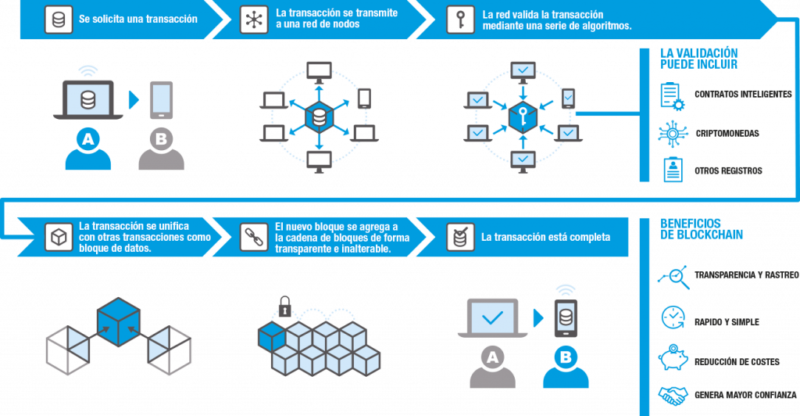
\includegraphics[width=.8\textwidth]{figures/funcionamientoblockchain.png}
    \label{fig:transaction}
\end{figure}
      
\subsubsection{Seguridad en Blockchain } 
La seguridad de la blockchain depende de varias capas de tecnología criptográfica y del diseño descentralizado de la red. Los elementos clave de su seguridad incluyen:
    \begin{enumerate}
        \item \textbf{Inmutabilidad}: Una vez que se agrega un bloque, es extremadamente difícil modificar los datos sin alterar el hash y afectar a todos los bloques posteriores. Cualquier intento de modificación sería rápidamente detectado por los nodos.
        \item \textbf{Distribución y descentralización}: Al distribuir el control de la red entre miles de nodos (en el caso de las redes más importantes), blockchain elimina los puntos de fallo únicos. Esto significa que, incluso si un nodo es comprometido o hackeado, el resto de la red sigue siendo seguro, de hecho dependiendo de los criterios de cada red, realmente mientras ente el 51 y 70 \% de nodos siga sin alterarse la red sigue siendo segura.
        \item \textbf{Criptografía de clave pública y privada}: Cada usuario de la red tiene una clave pública y una clave privada. La clave pública funciona como una dirección visible para recibir activos, mientras que la clave privada permite firmar transacciones, asegurando la autenticidad de la actividad en la red. Solo el propietario de la clave privada puede autorizar transacciones en nombre de su dirección pública protegiendo los fondos.
        \item \textbf{Hashing criptográfico}: El uso de algoritmos de \gls{hashing} (como \gls{sha256} en Bitcoin) convierte los datos de las transacciones en códigos únicos de longitud fija. Cualquier cambio en los datos originales generaría un hash completamente diferente, alertando a la red de la alteración. Este proceso es irreversible, lo que significa que el hash no puede descifrarse para revelar los datos originales.
    \end{enumerate}

Con todas estas características se puede afirmar que una red blockchain es una herramienta segura para la realización de transacciones monetarias y de reserva de valor. Ahora bien, ¿cómo se puede crear un sistema automatizado?. En redes como \gls{bitcoin}, el único tipo de operación que se puede realizar es el de transacción. Este proyecto se apoya en una red con capacidad de ejecutar \glspl{script} o como son llamados dentro de la red: \glspl{smartcontract}. \cite{[6]}


\subsection{Ethereum}
Ethereum es una plataforma de blockchain propuesta en 2013 por Vitalik Buterin a los 19 años de edad. \cite{[7]} Se ha escogido esta red principalmente por su capacidad  de despliegue de \glspl{smartcontract}, lo cual es necesario para este proyecto.

Aunque existen otras redes blockchain con capacidad de despliegue de \glspl{smartcontract}, como \citetitle{[9]} \cite{[9]} y \citetitle{[10]} \cite{[10]}, al tratarse de un proyecto basado en la economía \gls{defi} se ha seleccionado \gls{ethereum} debido a que su moneda es la que tiene mayor valor de mercado. Este se puede visualizar en la figura 2 a fecha de 14-03-2024 y a tiempo real en la web: \href{https://coinmarketcap.com/es/}{CoinMarketCap}\footnote{\href{https://coinmarketcap.com/es/}{https://coinmarketcap.com}.}

\begin{figure}[h]
    \centering
    \caption{Información a tiempo real del valor de criptomonedas, especialmente de  \citetitle{[9]} \cite{[9]}, \citetitle{[10]} \cite{[10]}, \citetitle{[7]} \cite{[7]} las cuales sí permiten la integración de \glspl{smartcontract}.}
    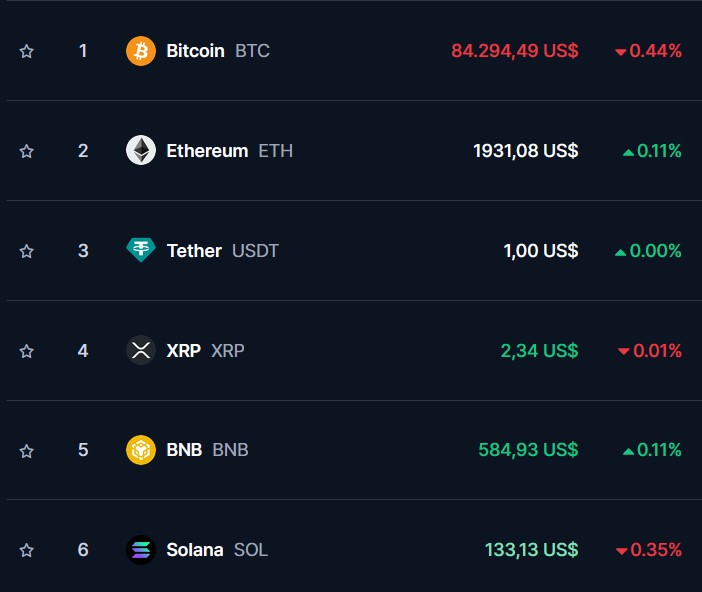
\includegraphics[width=.4\textwidth]{figures/coinmarket.jpg}
    \label{fig:criptovalues}
\end{figure}

Las principales características de  \gls{ethereum} y en las cuales se apoya este proyecto son:
    \begin{enumerate}
    
        \item \textbf{ Contratos Inteligentes y Máquina Virtual de Ethereum (\gls{evm})}
        La característica más destacada de Ethereum es su capacidad para ejecutar \gls{SC}. Estos son programas autoejecutables con condiciones predefinidas, que permiten automatizar una amplia variedad de procesos y acuerdos entre partes sin necesidad de intermediarios.
La Máquina Virtual de Ethereum (\gls{evm}) es la infraestructura que hace posible la ejecución de estos contratos inteligentes esta consiste en un entorno virtual que permite que el código de los Smart Contract se ejecute por igual y de manera segura en todos los nodos de la red Ethereum, lo que garantiza consistencia e inmutabilidad. La \gls{evm} también es compatible con varios lenguajes de programación, siendo \gls{solidity} el más utilizado para desarrollar contratos inteligentes en la red.
        \item \textbf{Plataforma para \glspl{dapp}} Ethereum fue la primera blockchain en introducir el concepto de aplicaciones descentralizadas (\glspl{dapp}). Las \glspl{dapp} son aplicaciones que funcionan en redes descentralizadas, permitiendo que los usuarios interactúen de manera directa y sin intermediarios en diferentes servicios, desde finanzas hasta juegos y redes sociales.
        
Gracias a los contratos inteligentes y la \gls{evm}, Ethereum se convirtió en una plataforma que permite a los desarrolladores crear y desplegar sus propias aplicaciones sobre la misma red, similar a una "\gls{appstore}" descentralizada. Esto le ha dado una gran popularidad y ha impulsado el crecimiento de sectores como las finanzas descentralizadas (\gls{defi}) y los tokens no fungibles (\gls{nft}), lo que ha ampliado las posibilidades de uso de blockchain más allá de las transferencias de valor.

        \item \textbf{ Criptoeconomía y Modelo de Tokenización}
         Otra diferencia clave es que Ethereum cuenta con su propia criptomoneda,
          Ether (\gls{eth}), que es necesaria para realizar transacciones y pagar las comisiones para obligatorias
          para ejecutar \gls{smartcontract}en la red.
          La comisión cobrada para cada transacción se calcula según la cantidad de \gls{gas} muliplicado por su precio 
           en el momento de la transacción.
          El  \gls{gas} mide el trabajo computacional necesario para ejecutar una operación en la red.
          Estas comisiones son parcialmente transferidas a los  nodos mineros o nodos validadores, incentivando a estos
          a verificar las transacciones  mantenienod la red segura y operativa.
          La parte de la comisión que no es transferida a los nodos que participan en la red es retirada de la red.

          Además, Ethereum introdujo el concepto de  \enquote{tokenización}, esto permite representar activos o derechos a través de \gls{token}.
          Para facilitar el uso y transferencia de estos, se han creado distintos estandares como por ejemplo:
          \begin{enumerate}
            \item \gls{erc-20}: tokens fungibles, cuyas unidades son intercambiables entre sí, como puede ser una criptomenda.
            \item \gls{erc-721} tokens no fungibles, que permiten distinguir cada token individualmente, pudiendose usar para representar
                 activos en la vida real o distintos derechos de usuario como una votación.
            \item \gls{erc-1155}ERC-1155: permite gestionar distintos tipos de tokens en una misma operación,
             tanto fungibles como no fungibles, en un mismo contrato.
          \end{enumerate}

        \item \textbf{Identidad} Ethereum es una red descentralizada, no utiliza identificaciones centralizadas como puede ser la centralización estatal del \gls{dni}.
        Aunque no es una característica exclusiva de Ethereum. el sistema de identificación de esta red consiste en el típico sistema asimétrico de clave pública y privada de forma que para identificar a cada usuario se utiliza su clave pública y para que este pueda ejecutar transacciones en su nombre utiliza su clave única y privada.
        Sin embargo, esto también significa que no hay una forma nativa de verificar identidades del mundo real.
        
        \item \textbf{Oráculos} son servicios externos que alimentan la blockchain con datos de fuentes externas, permitiendo que los contratos inteligentes interactúen con el mundo real. Por ejemplo, en aplicaciones \gls{defi} relacionadas con bienes raíces, un oráculo podría verificar que una propiedad física corresponde a un token en Ethereum, permitiendo así transacciones con respaldo en activos físicos.
    
    \end{enumerate}

Se puede concluir que ethereum es un buen  medio para  desarrollar la intencionalidad del proyecto gracias a su \gls{evm} y la posiblidad de definir contratos inteligentes en ella, utilizando como moneda de cambio \gls{eth} e icluso añadir avales a los contratos y préstamos a través de los \gls{nft} y oráculos que los identifican en el mundo físico.

\paragraph{Sepholia ETH}
Sepolia\cite{[21]}es una red de pruebas que permite a los desarrolladores experimentar y probar contratos inteligentes y aplicaciones descentralizadas en un entorno que simula la red principal de Ethereum pero sin utilizar Ether real.
Para obtener SepoliaETH, los desarrolladores pueden utilizar faucets como Sepoliafaucet\cite{[22]}, que son servicios que proporcionan pequeñas cantidades de esta criptomoneda de prueba de forma gratuita.

\section{Tecnologías para el desarrollo}

\subsection{Identificación en la red: Metamask}

En una red blockchain los usuarios interactúan con la red mediante direcciones, estas direcciones no permiten conocer
directamente la identidad de la persona que la utiliza. 
Una cuenta en Metamask permite que un usuario guarde en un mismo punto todas las direcciones que utiliza para comunicarse
con las redes blockchain, este sistema recibe el nombre de \gls{wallet} o cartera de direcciones.
Aunque Metamask no relacione directamente sus cuentas con personas físicas, permite identifiar al usuario dentro de las 
aplicaciones descentralizadas (\gls{dapp}).
Metamask además ofrece librerías capaces de interactuar directamente con las funciones \gls{web3} siendo una buena opción
para delegar el sistema de identificacón

Encontramos distintas alternativas como Coinbase\cite{[11]} y RabbyWallet\cite{[12]} 
pero para este proyecto se ha decido hacer uso de  Metamask\cite{[13]} debido a su mayor
 popularidad y sobretodo la facilidad de acceso a nivel de usuario. \citetitle{[14]} \cite{[14]}

Metamask es una extensión del navegador a través la cual una \gls{dapp} usando librerías \gls{web3} puede detectar
 e identificar al  usuario en el sistema siempre que este de su autorización. 

A demás metamask también es un asistente para revisar y firmar transacciones y operaciones con \gls{smartcontract}
que requieren de una dirección privada, como, en el caso de este sistema, la solicitud de un prestamo.

Estas caracteríscas hace de Metamask una  herrammienta muy potente para delegar un servicio tan delicado como la 
identificación del usuario.

\subsection{Web3}

Se le llama web3 a la próxima generación web (actual web2).
Entre otras cosas buscará la descentralización y sobretodo el uso de \gls{dapp}.
A su vez web3 es un \gls{framework} de \gls{javascript} que permite acciones como 
conectarte a una red bockchain, gestionar cuentas, firmar transacciones, consultar saldos de las cuentas, interactuar con \glspl{smartcontract}.
Este framework abstrae la complejidad de las interacciones con la blockchain, simplificando el desarrollo de \glspl{dapp}.

\subsection{Solidity}
Solidity\cite{[15]} es un lenguaje de programación diseñado para escribir contratos inteligentes que se ejecutan en la blockchain de Ethereum. Es similar a JavaScript y C++, con características específicas para gestionar transacciones, almacenamiento en blockchain y lógica descentralizada. Es fundamental para desarrollar aplicaciones descentralizadas (dApps) y sistemas DeFi.

\subsection{Remix IDE}
Remix Project \cite{[16]} es el conjunto de herramientas más exhausitivo que puede usarse para toda la experiencia de desarrollo de  \glspl{smartcontract}  para  usuarios de cualquier nivel de conocimientos y como laboratorio de aprendizaje para enseñar y experimentar con Ethereum.
También es deal como asistente de compilación y despliegue  de \glspl{smartcontract} en \gls{ethereum}.

\subsection{Node.js}
Node.js \cite{[17]}entorno de ejecución \gls{javascript}  de código abierto y gratuito que facilita la incorporación de paquetes a un proyecto. Muy utilizado para instalar y utilizar librerías  web3.

\subsection{Angular}
\citetitle{[33]} es un framework de código abierto basado en TypeScript..
Sus herramientas hacen más sencillo las tareas comunes al desarrollo web como la gestión de rutas de dirección,
organización de código a través de elementos llamados \enquote{componentes}, recogida de datos de usuario, etc..


\subsection{Ionic}
\citetitle{[32]} es un framework de código abierto orientado en el desarrollo de los componentes visuales en una
aplicación web. En combinación con \citetitle{[33]} es una herramienta que facilita mucho
el desarrollo. 

\subsection{Mochatest Framework}
\label{sec:mochasection}
Marco de pruebas en \gls{javascript} diseñado para ejecutar pruebas unitarias y de integración en aplicaciones Node.js. Ofrece una estructura flexible, con soporte para pruebas síncronas y asíncronas.

\subsection{Truffle}
Truffle \cite{[18]} es un conjunto de herramientas para el desarrollo de aplicaciones en Ethereum.
Principalmente puede compilar \glspl{smartcontract} y obtener información necesaria para su despliegue en la red.
Truffle también tiene una herramienta muy poderosa: Ganache \cite{[19]}, esta es capaz de ejecutar  una \gls{evm} en un entorno local. Perfecto para el desarrollo aunque con tendencia a fallos.

\subsection{Explorador de bloques Etherscan}
Etherscan\cite{[20]} es un explorador de blockchain para Ethereum que permite visualizar transacciones, contratos inteligentes, balances de wallets y otra información en tiempo real. Es una herramienta clave para analizar y verificar actividades en la red Ethereum.



\chapter{Arquitectura y desarrollo}
\label{ch:arquitecturaydesarrollo}
\section{Solución propuesta}

Este proyecto propone una \gls{dapp} que gestiona préstamos de \gls{eth} dentro 
de la red \gls{ethereum} a través de \gls{smartcontract} desplegados en dicha
red.

Como se ha explicado en la comparación con otros protocolos \gls{defi}, 
la diferenciación de este sistema es que solo una entidad, poseedora del proyecto,
está autorizada a ofrecer los préstamos, configurar los tipos de préstamos
disponibles y gestionar los fondos.

El sistema se basa en \glspl{smartcontract} que registran en la red la
información necesaria para gestionar los préstamos. Estos contratos permiten
automatizar parte de la gestión y conservar un historial de las operaciones.

El usuario de la \gls{dapp} interactúa con el sistema a través de una interfaz web
en la que conectando su cartera con \gls{metamask} puede gestionar sus propios 
préstamos sin la necesidad de interactuar directamente con la organización del 
sistema.

El seguimiento de control de pagos de los contratos 
funciona como una máquina de estados automatizada que es accionada como un 
semáforo con ciclos mensuales.

En la figura~\ref{fig:semaforos} se pueden ver los tres tipos de estados en los que
puede encontrarse un préstamo al chequeo mensual de pagos (estado 0), cómo actúa la
\gls{dapp} dependiendo de su estado durante el chequeo (estado 1), y cómo queda
el préstamo pasado el chequeo esperando al próximo (estado 0).

\begin{figure}[H]
    \centering
    \caption{Diagrama de estados que asegura el control de
    los contratos del sistema.}
    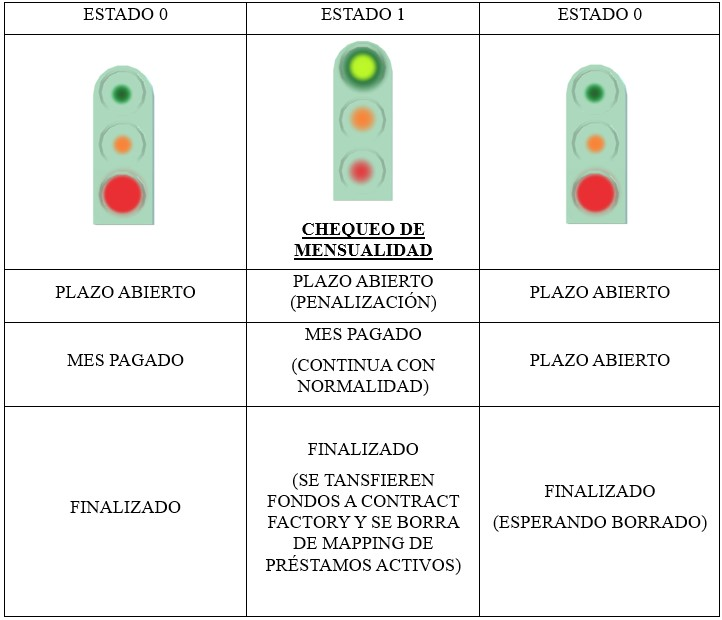
\includegraphics[width=\textwidth]{figures/semaforos.jpg}
    \label{fig:semaforos}
\end{figure}



\section{Limitaciones del proyecto}
\subsection{Limitaciones legales}
\label{subsec:limitaciones-legales}

Durante este proceso de desarrollo, en diciembre de 2024, la Unión Europea aprueba 
el Reglamento Europeo de Criptoactivos~\cite{[24]}. 
El objetivo de este reglamento es establecer normas para las entidades emisoras
y proveedoras de servicios relacionados con la criptoactividad.

En el nuevo reglamento se  tratan distintas cuestiones entre las que se 
encuentran:
\begin{enumerate}
    \item Requisitos de transparencia absoluta a las plataformas de negociación 
    de criptoactivos.
    \item Necesidad de autorización europea para la emisión y provisionamiento
    de criptoactivos.
    \item Protección del valor monetario en euros de los clientes.
    \item Creación de medidas de control de las operaciones con información 
    privilegiada y manipulación de mercado.
\end{enumerate}

En esta normativa se especifican acciones obligatorias para entidades financieras 
que pueden adoptar este proyecto. Dentro de estas acciones se definen elementos 
comunes a cualquier empresa como definirse como persona jurídica o actuar de forma 
honesta, justa y profesional.

Una de las exigencias que pueden limitar el proyecto es la obligatoriedad de ofrecer
la capacidad de convertir en euros los criptoactivos proporcionados por este
proyecto. Específicamente se obliga a mantener:
\begin{enumerate}
    \item Un fondo propio de 350\,000~\texteuro{}
    \item El 2\% del importe medio de los activos de reserva
    \item Una cuarta parte de los gastos generales fijos del año anterior
    \item Establecimiento de planes de recuperación y reembolso en caso de no 
    cumplir las obligaciones de la normativa 
\end{enumerate}

Estas acciones obligan a cualquier entidad que quiera hacer uso de este proyecto 
a aprovisionar las cantidades definidas en la normativa.

\subsection{Limitaciones técnicas}

El sistema desarrollado presenta una serie de limitaciones técnicas derivadas 
tanto del alcance definido para el proyecto como de las características propias de 
una solución basada en \glspl{smartcontract}. Las principales
limitaciones identificadas son las siguientes:

\begin{enumerate}
    \item \textbf{Pagos anticipados:} el sistema no contempla actualmente la
    realización de pagos anticipados sobre los préstamos contratados.

    \item \textbf{Cancelación anticipada:} no se contempla la posibilidad de
    cancelar un préstamo antes de que finalice el periodo establecido inicialmente
    en el momento de su contratación.

    \item \textbf{Ausencia de garantías o colateral:} el sistema no incorpora
    mecanismos de colateralización que permitan garantizar el pago del préstamo
    en caso de impago.

    \item \textbf{Uso de un único activo:} el prototipo utiliza exclusivamente
    \gls{eth} como activo para la concesión y devolución de los préstamos.
    No se contempla actualmente el uso de otros tokens o activos digitales como
    unidad de préstamo.

    \item \textbf{Escalabilidad y consumo de \gls{gas}:} el incremento del
    número de préstamos activos implica un mayor número de operaciones que deben
    ser procesadas y registradas en la \gls{blockchain}. En consecuencia, el coste
    acumulado de \gls{gas} puede aumentar a medida que crece el volumen de
    préstamos gestionados. Esta situación no tiene por qué invalidar el proyecto, pero sí exige un desarrollo orientado a mejorar su escalabilidad.
    \end{enumerate}

Estas limitaciones deben tenerse en cuenta al valorar una posible aplicación del
sistema en un entorno real a la vez que se plantean como líneas de desarrollo 
futuro.

\section{Análisis y diseño del software}
En esta sección se muestran diagramas y tablas que definen la estructura y 
el flujo del sistema.

\subsection{Actores del sistema}
Los actores que pueden participar en el sistema son:

\begin{itemize}
    \item \textbf{Usuario prestatario (User):} Usuario que accede al servicio de
    préstamos.
    \item \textbf{Entidad prestamista (Owner):} Entidad que ofrece los distintos
    tipos de préstamos.
\end{itemize}

\subsubsection{Diagrama UML}
En la figura~\ref{fig:uml} hay representado un \gls{diagramauml}
que relaciona los actores del sistema con los 
\enquote{Casos de Uso} que pueden realizar.

\begin{figure}[H]
    \centering
    \caption{Diagrama UML representando los actores del sistema relacionados 
    con los casos de uso a los que tienen acceso.}
    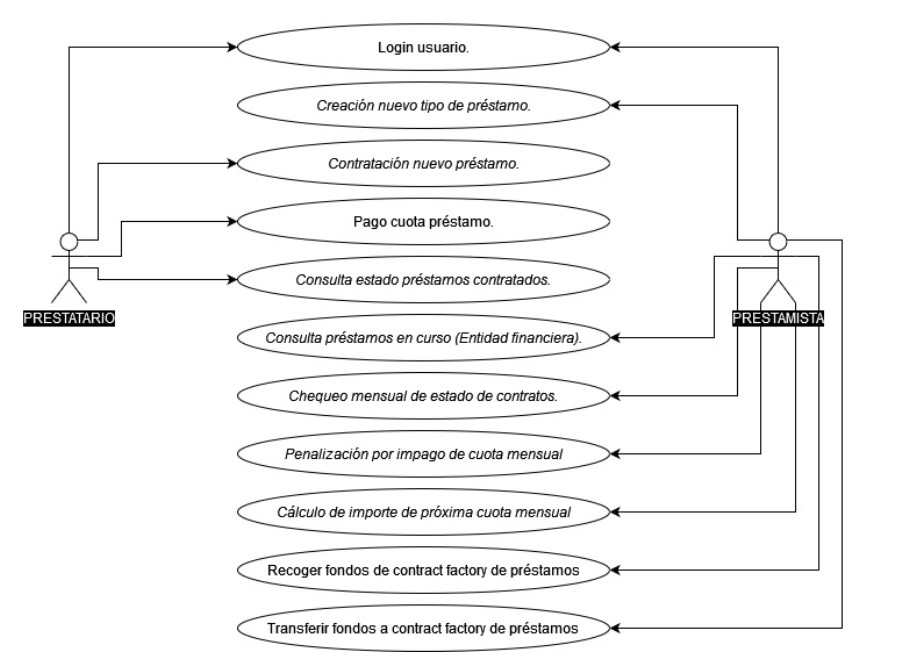
\includegraphics[width=\textwidth]{figures/uml.jpg}
    \label{fig:uml}
\end{figure}

\subsubsection{Diagrama de secuencia UML}
Para mostrar cómo interactúan los actores con el sistema en una línea de tiempo
y conocer el flujo de información que sucede en el sistema se ha definido
el siguiente \gls{secuenciauml} en la figura~\ref{fig:secuenciauml}.

En este caso, el diagrama de secuencia muestra cómo todo registro en el sistema
siempre es grabado en la \gls{blockchain}, siendo un flujo clave en este proyecto 
para poder dar las propiedades de veracidad e inmutabilidad a la información de los
préstamos.

\begin{figure}[H]
    \centering
    \caption{Diagrama de secuencia que representa cómo la información
    vital del sistema queda registrada en la red aportando las características 
    de inmutabilidad y confianza propias del proyecto.}
    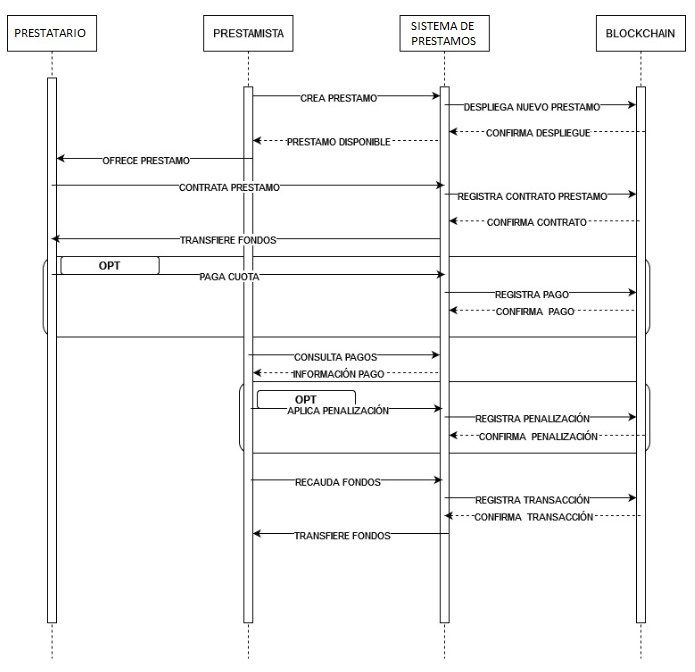
\includegraphics[width=\textwidth]{figures/diagramasecuencia.jpg}
    \label{fig:secuenciauml}
\end{figure}

\subsection{Casos de uso}

En el marco del desarrollo del presente proyecto, 
se ha priorizado la definición de un conjunto de casos de uso que representan 
los escenarios esenciales para cumplir con los objetivos fundamentales del 
sistema, de acuerdo con el alcance limitado del proyecto.

La selección de los casos de uso  no pretende abarcar una totalidad 
de posibles funcionalidades del sistema sino un conjunto operativo sólido y 
funcional, comentando también un posible desarrollo futuro.

Estos casos de uso se definen en las tablas ~\ref{tab:casos-uso-sistema} y 
~\ref{tab:casos-uso-posteriores}.

\subsubsection{Pantallas del sistema}
Para facilitar la comprensión de los casos de uso, se enumeran las principales
pantallas del sistema:

\begin{itemize}
    \item \textbf{Pantalla principal común:} Pantalla de inicio común a todos los
    usuarios, principalmente para identificarse en el sistema.
    \item \textbf{Pantalla principal del prestamista.}
    \item \textbf{Pantalla principal del prestatario.}
\end{itemize}

\subsubsection{Casos de uso}
\begin{table}[H]
\centering
\caption{Casos de uso del sistema}
\label{tab:casos-uso-sistema}
\small
\begin{tabular}{|c|l|c|c|}
    \hline
    \rowcolor[HTML]{D0E7FF}
    Código  & Descripción   & Prioridad & Dependencia  \\ \hline
    CU1     & Inicio de sesión usuario        & 10   &   \\ \hline
    CU2     & Creación nuevo tipo de préstamo     & 9   &   \\ \hline
    CU3     & Contratación nuevo préstamo        & 8   &  CU2 \\ \hline
    CU4     & Consulta estado préstamos contratados        & 7   & CU3   \\ \hline
    CU5     & Pago cuota préstamo       & 6   & CU3 \\ \hline
    CU6     & Consulta préstamos en curso (Entidad prestamista)        & 5   & CU3 \\ \hline
    CU7     & Chequeo mensual de estado de contratos        & 4   &   \\ \hline
    CU8     & Penalización por impago de cuota mensual       & 3   &CU7   \\ \hline
    CU9     & Cálculo de importe de próxima cuota mensual         & 2   &  CU3  \\ \hline
    CU10     & Retirar fondos del sistema        & 1   &   \\ \hline
    CU11     & Ingresar fondos en el sistema        & 1   &   \\ \hline
\end{tabular}
\end{table}


\subsubsection{Casos de uso para posteriores desarrollos}


    \begin{table}[H]
    \centering
    \caption{Casos de uso para desarrollos posteriores}
    \label{tab:casos-uso-posteriores}
    \begin{tabular}{|c|l|}
        \hline
        \rowcolor[HTML]{D0E7FF}
    Código & Descripción \\ \hline
    \hypertarget{cu:garantia}{CU12}
        & Garantía de devolución en caso de impago \\ \hline
    \hypertarget{cu:euribor}{CU13}
        & Consulta del valor del \gls{euribor} \\ \hline
    \hypertarget{cu:solvencia}{CU14}
        & Validación de solvencia económica de usuarios \\ \hline
    \end{tabular}
    \end{table}

\subsubsection{Casos de uso detallados}
En esta sección se describen los casos de uso implementados y más adelante,
en la sección de trabajo futuro se comentarán los casos de uso futuros.

\begin{table}[H]
\centering
\caption{Casos de uso 1}
\begin{tabular}{|c|p{12cm}|}
    \hline
    \rowcolor[HTML]{D0E7FF}
    CU1 & \gls{login} del usuario. \\ \hline
    Descripción   & Los usuarios se identificarán en el sistema a través de MetaMask.  \\ \hline
    Pantalla     & Pantalla inicial. (Se redirecciona a esta página si no se ha realizado el \gls{login}).   \\ \hline
    Rol     & Cualquier usuario. \\ \hline
    Flujo     &    - El usuario, al acceder a la página web, recibirá una notificación
    por parte de MetaMask  para poder acceder al
                           servicio. \newline
                   - La extensión de MetaMask permite la autenticación del          usuario y la página se redirige a la página correspondiente a su rol.
    \\ \hline
\end{tabular}
\end{table}

\begin{table}[H]
\centering
\caption{Casos de uso 2}
\begin{tabular}{|c|p{12cm}|}
    \hline
    \rowcolor[HTML]{D0E7FF}
    CU2 & Creación nuevo tipo de préstamo. \\ \hline
    Descripción   & La entidad prestamista puede crear nuevos productos tipo \enquote{préstamo}.  \\ \hline
    Pantalla     & Pantalla principal de la entidad prestamista.  \\ \hline
    Rol     & Owner. \\ \hline
    Flujo     &    - El usuario owner tiene un formulario en su página principal para
rellenar la información necesaria para la creación de un nuevo tipo de
préstamo.\newline
                   - Este contrato se le mostrará al usuario prestatario en su página principal en forma de producto para contratar.
                 \\ \hline
\end{tabular}
\end{table}

\begin{table}[H]
\centering
\caption{Casos de uso 3}
\begin{tabular}{|c|p{12cm}|}
    \hline
    \rowcolor[HTML]{D0E7FF}
    CU3 & Contratación nuevo préstamo. \\ \hline
    Descripción   & Los usuarios prestatarios pueden seleccionar el préstamo que desean contratar.  \\ \hline
    Pantalla     & Pantalla principal de usuarios prestatarios.   \\ \hline
    Rol     & User. \\ \hline
    Flujo     &    - En la página principal el usuario podrá visualizar los posibles préstamos que
puede contratar. \newline
                   - El usuario contrata un nuevo préstamo pinchando en el botón de
\enquote{Contratar}. \newline
                                 Tan pronto como se procese la transacción, la \gls{dapp} llamará al \gls{smartcontract} desplegado en la red el cual genera otro \gls{smartcontract} que refleja el estado del préstamo en
cada momento. \newline
                                Al mismo tiempo, las unidades de \gls{eth} solicitadas en el préstamo serán transferidas
automáticamente desde los fondos del \gls{smartcontract} que conserva el balance del sistema a la dirección del
usuario.
                  \\ \hline
\end{tabular}
\end{table}

\begin{table}[H]
\centering
\caption{Casos de uso 4}
\begin{tabular}{|c|p{12cm}|}
    \hline
    \rowcolor[HTML]{D0E7FF}
    CU4 & Consulta estado préstamos contratados. \\ \hline
    Descripción   & Los usuarios del servicio podrán consultar el estado de sus préstamos contratados
visualizándolos en su página principal.  \\ \hline
    Pantalla     & Pantalla principal usuario.   \\ \hline
    Rol     & User. \\ \hline
    Flujo     &    En el momento en que el usuario hace inicio de sesión ya puede visualizar los contratos
que tiene contratados. \\ \hline
                 
\end{tabular}
\end{table}

\begin{table}[H]
    \centering
    \caption{Casos de uso 5}
\begin{tabular}{|c|p{12cm}|}
    \hline
    \rowcolor[HTML]{D0E7FF}
    CU5 & Pago cuota préstamo. \\ \hline
    Descripción   & Los usuarios del servicio de préstamo realizan el pago de sus 
    mensualidades a través de la \gls{dapp} del proyecto.  \\ \hline
    Pantalla     & Pantalla principal de usuarios prestatarios.   \\ \hline
    Rol     & User. \\ \hline
    Flujo     &    - En la página principal del usuario aparecen los distintos préstamos que
tiene contratados y sus respectivos estados, junto a esto, existe un botón para
cada contrato que transfiere la mensualidad calculada previamente desde la
cuenta del usuario a la dirección del \gls{smartcontract} de préstamo.
                 \\ \hline
\end{tabular}
\end{table}

\begin{table}[H]
\centering
\caption{Casos de uso 6}
\begin{tabular}{|c|p{12cm}|}
    \hline
    \rowcolor[HTML]{D0E7FF}
    CU6 & Consulta préstamos en curso (Entidad prestamista). \\ \hline
    Descripción   & La entidad prestamista puede consultar el estado de cada préstamo en
curso. \\ \hline
    Pantalla     &Pantalla principal de la entidad prestamista.  \\ \hline
    Rol     & Owner. \\ \hline
    Flujo     &    - En la página principal del propietario aparecen los contratos en curso.
                 \\ \hline
\end{tabular}
\end{table}

\begin{table}[H]
\centering
\caption{Casos de uso 7}
\begin{tabular}{|c|p{12cm}|}
    \hline
    \rowcolor[HTML]{D0E7FF}
    CU7 & Chequeo mensual de estado de contratos. \\ \hline
    Descripción   & La entidad prestamista ejecuta la orden de comprobar qué mensualidades no
han sido pagadas ese mes.  \\ \hline
    Pantalla     & Pantalla principal de entidad prestamista. \\ \hline
    Rol     & Owner. \\ \hline
    Flujo     &    Desde la página principal del propietario se tiene acceso al botón que lanza
esa orden siempre y cuando hayan pasado 30 días desde la última orden.
                 \\ \hline
\end{tabular}
\end{table}

\begin{table}[H]
\centering
\caption{Casos de uso 8}
\begin{tabular}{|c|p{12cm}|}
    \hline
    \rowcolor[HTML]{D0E7FF}
    CU8 & Penalización por impago de cuota mensual. \\ \hline
    Descripción   & Los contratos en estado de impago generan una penalización de deuda, esta
penalización solo puede suceder una vez al mes.  \\ \hline
    Pantalla     & Pantalla principal de entidad prestamista.  \\ \hline
    Rol     & Owner. \\ \hline
    Flujo     &    Cuando el propietario genera la orden de chequeo mensual los contratos
que tengan estado de \enquote{impago} aumentarán su valor de deuda.
                 \\ \hline
\end{tabular}
\end{table}

\begin{table}[H]
\centering
\caption{Casos de uso 9}
\begin{tabular}{|c|p{12cm}|}
    \hline
    \rowcolor[HTML]{D0E7FF}
    CU9 & Cálculo de importe de próxima cuota mensual. \\ \hline
    Descripción   & El importe de la próxima cuota mensual es un valor dinámico sujeto a
penalizaciones.  \\ \hline
    Pantalla     & Pantalla principal usuario.  \\ \hline
    Rol     & User. \\ \hline
    Flujo     &    - Tras el chequeo mensual la cuota del próximo pago se podrá ver
modificada en caso de penalización. \newline
                   - En la información de los préstamos contratados aparecerá la cantidad de la
cuota del mes en curso.
                 \\ \hline
\end{tabular}
\end{table}

\begin{table}[H]
\centering
\caption{Casos de uso 10}
\begin{tabular}{|c|p{12cm}|}
    \hline
    \rowcolor[HTML]{D0E7FF}
    CU10 & Retirar fondos del sistema. \\ \hline
    Descripción   & La entidad prestamista propietaria  del sistema de préstamos puede disponer de los fondos almacenados en el sistema
cuando desee.  \\ \hline
    Pantalla     & Pantalla principal de Owner.   \\ \hline
    Rol     & Owner. \\ \hline
    Flujo     &    La entidad prestamista tendrá una casilla en su página principal para escribir y recibir el
importe desde la dirección del \gls{smartcontract} con el balance a su dirección de la red.
                 \\ \hline
\end{tabular}
\end{table}

\begin{table}[H]
\centering
\caption{Casos de uso 11}
\begin{tabular}{|c|p{12cm}|}
    \hline
    \rowcolor[HTML]{D0E7FF}
    CU11 & Ingresar fondos en el sistema. \\ \hline
    Descripción   & La entidad prestamista  puede transferir cualquier cantidad de \gls{eth}
    al sistema de préstamos para mantener
 un saldo positivo y poder realizar estos préstamos.\\ \hline
    Pantalla     & Pantalla principal Owner.   \\ \hline
    Rol     & Owner. \\ \hline
    Flujo     &    La entidad tendrá una casilla en su página principal para escribir y transferir el
importe deseado a la dirección del sistema de préstamos.
                 \\ \hline
\end{tabular}
\end{table}

\clearpage
\subsection{Entidades del sistema}
A continuación se definen las entidades cuyas relaciones compondrán y 
habilitarán las funciones del sistema propuesto.

\begin{table}[H]
\centering
\caption{Definición de entidades del sistema}
\begin{tabular}{|c|p{12cm}|}
    \hline
    \rowcolor[HTML]{D0E7FF}
    1 & Usuario. \\ \hline
    Descripción   & Usuario que accede al servicio de préstamos.  \\ \hline
    Atributos     & Dirección pública de la red.   \\ \hline
    Acciones     &- Pedir préstamo.  \newline
                    - Pagar préstamo.\\ \hline

    \hline
    \rowcolor[HTML]{D0E7FF}
    2 & Propietario. \\ \hline
    Descripción   & Propietario del sistema, único capaz de recolectar los fondos del sistema. Normalmente una entidad prestamista.  \\ \hline
    Atributos     & Dirección pública de la red.   \\ \hline
    Acciones     &- Transferir unidades al sistema. \newline
                    - Recoger unidades del sistema.\\ \hline
   

    \hline
    \rowcolor[HTML]{D0E7FF}
    3 & Sistema de préstamos.     \\ \hline
    Descripción   & Conjunto de \glspl{smartcontract} que definen los elementos del sistema y cuya ejecución valida las transacciones del sistema.  \\ \hline
    Atributos     &- Dirección de propietario. \newline
                    - Lista de préstamos contratables. \newline
                    - Lista de usuarios junto con sus préstamos en curso.\\ \hline
    Acciones     & - Ejecutar las transacciones ordenadas por los usuarios del sistema.  \newline
                    - Registrar en la red \gls{ethereum} la información del sistema.\\ \hline
   
\end{tabular}
\end{table}

\clearpage
\subsubsection{Diagrama de entidad-relación}
El  diagrama  representado en la figura~\ref{fig:er} pretende 
definir mediante relaciones entre las entidades las funciones que 
definen el sistema.
\begin{figure}[H]
    \centering
    \caption{Diagrama de entidad-relación.}
    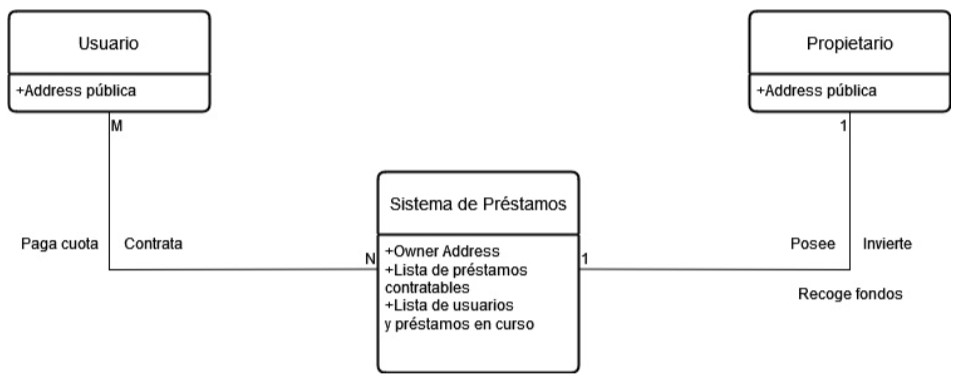
\includegraphics[width=\textwidth]{figures/E-R.jpg}
    \label{fig:er}
\end{figure}

\section{Análisis de los contratos inteligentes implicados}

En esta sección se define la arquitectura de diseño utilizada para los 
\glspl{smartcontract}, así como los atributos (tablas~\ref{fig:atributosfactory} y \ref{fig:atributosprestamo}) y 
funciones (tablas~\ref{fig:funcionesfactory} y \ref{fig:funcionesprestamo}) de 
cada uno de ellos.

\subsection{Diagrama de entidad-relación de contratos inteligentes}

Aunque no sean entidades del sistema, para explicar detalladamente la arquitectura 
de diseño se define otro diagrama de entidad-relación en la
figura~\ref{fig:ersmartcontract}.

\begin{figure}[H]
    \centering
    \caption{Diagrama de entidad-relación que representa las relaciones y funciones entre los contratos inteligentes.}
    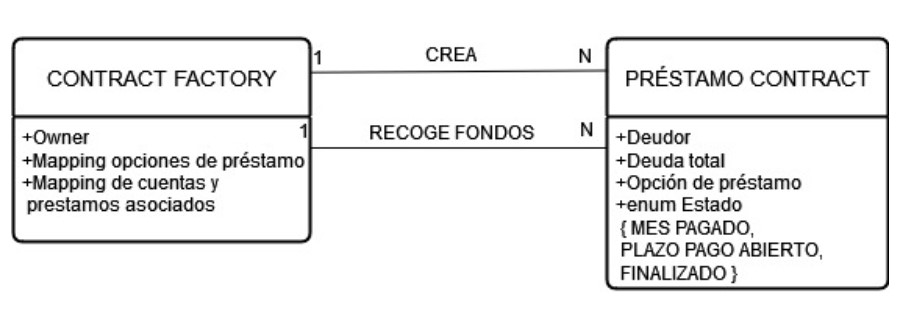
\includegraphics[width=\textwidth]{figures/E-R-smartcontracts.jpg}
    \label{fig:ersmartcontract}
\end{figure}
\subsubsection{PrestamosFactory}
La figura~\ref{fig:ersmartcontract} también define gráficamente el
patrón de diseño utilizado en el desarrollo de los \glspl{smartcontract}. A este
patrón se le denomina \enquote{Factory}.

El diseño de \enquote{Factory} encaja perfectamente en el desarrollo
de este proyecto ya 
que nos permite crear los distintos contratos de préstamo
de forma dinámica y automática.
En esta arquitectura, un contrato principal (el \textit{Factory}) actúa como 
intermediario recibiendo las solicitudes y generando nuevos contratos 
(\textit{contratos préstamo}) según
las necesidades de los usuarios o la aplicación.
Dentro de este contrato se definen los distintos tipos de préstamos que pueden 
ser contratados por los usuarios,
así como las distintas funcionalidades de gestión y monitorización.
Para ello este contrato cuenta con variables como las del fragmento de código siguiente:
\begin{lstlisting}[language=Solidity, caption={Registro de préstamos en curso por usuario},label={lst:prestamoscursando}]
    mapping(address => PrestamoCursando[])  prestamosCursando;
    address[] clientes;
\end{lstlisting}
En el fragmento de código del listado~\ref{lst:prestamoscursando} se observa 
la variable \textit{prestamosCursando} perteneciente al \gls{smartcontract} principal
\textit{PrestamosFactory}, la cual guarda en la red \gls{blockchain} el
conjunto de direcciones correspondientes a un contrato tipo \textit{Préstamo} 
pertenecientes al sistema.

Por otra parte, cada contrato creado por \textit{PrestamosFactory}, es decir, cada contrato de préstamo, mantiene información específica como la dirección
del prestatario, la deuda restante, el número de cuotas pendientes, 
el estado del préstamo o el porcentaje de penalización aplicable, tal y como 
se muestra en el fragmento de código~\ref{lst:prestamovariables}.



        \begin{lstlisting}[language=Solidity, 
            caption={Variables contrato préstamo},
            label={lst:prestamovariables}]
            uint index;
            enum State { PAGADO, ABIERTO, FINALIZADO }
            State state;
            address prestatario;
            address entidadFinanciera;
            address payable prestamosFactory;
            uint256 cuotasRestantes;
            uint256 cantidadPrestada;
            uint256 deudaRestante;
            uint256 cuotaMensual;
            uint256 penalizacion;
            uint256 ultimoCheckeo;
        \end{lstlisting}



\subsection{Análisis de contratos inteligentes}
\subsubsection{PrestamosFactory }
El contrato \textit{PrestamosFactory} centraliza la gestión de los tipos de
préstamo disponibles y el registro de los préstamos asociados a cada usuario. 
Para ello, mantiene un conjunto de atributos que identifican al propietario del 
sistema, definen las condiciones de los productos y 
relacionan a los usuarios con sus contratos de préstamo. 
La tabla~\ref{fig:atributosfactory} recoge estos atributos.
    \begin{table}[H]
    \centering
    \caption{Descripción de atributos del Contrato PrestamosFactory}
        \label{fig:atributosfactory}
    \small
    \begin{tabular}{|p{3cm}|p{4.1cm}|p{6.1cm}|}
        \hline
        \rowcolor[HTML]{D0E7FF}
        Nombre & Tipo de dato & Descripción\\ \hline
        Owner&\gls{addresstype}&Dirección de la red \gls{ethereum} perteneciente a la 
        propietaria del sistema.\\ \hline
        Tipos de préstamo&\texttt{TipoContrato[]}&Array que guarda los tipos de préstamo contratables por el usuario. \newline
    Esta variable solo puede ser editada si el usuario se identifica con la dirección del propietario.\\ \hline
    TipoPréstamo&Struct&Conjunto de variables que definen un tipo de préstamo (importe, intereses, deuda total, penalización de impago y  cuotas)\\ \hline
    Préstamos en curso&\texttt{mapping(address =>}\newline\texttt{Prestamo\allowbreak{}Cursando[])}&Mapping que relaciona la dirección de un
    usuario con las direcciones de sus
    préstamos en curso. \newline
    El contrato principal actualiza este registro al contratar o eliminar un préstamo.\\ \hline
    \end{tabular}
    \end{table}


A continuación, la tabla~\ref{fig:funcionesfactory} presenta las funciones del contrato
\textit{PrestamosFactory}, sus parámetros de entrada y salida y una
descripción de su finalidad.

\begin{table}[H]
\centering
\caption{Descripción de funciones del Contrato PrestamosFactory}
\label{fig:funcionesfactory}
\small
\begin{tabular}{|p{3.5cm}|p{3cm}|p{2.1cm}|p{4.4cm}|}
\hline
\rowcolor[HTML]{D0E7FF}
Nombre & Entrada & Salida & Descripción \\ \hline
\texttt{definir\allowbreak{}Prestamo} & Interés, importe, cuotas y penalización & --- & Crea un tipo de préstamo y emite el evento correspondiente. Solo puede ejecutarla el propietario. \\ \hline
\texttt{contratar\allowbreak{}Prestamo} & Prestatario e índice del tipo & --- & Crea un contrato individual, lo registra y transfiere el importe al prestatario. \\ \hline
\texttt{get\allowbreak{}Clientes} & --- & Direcciones & Devuelve las direcciones de los clientes registrados. Solo puede consultarlas el propietario. \\ \hline
\texttt{recolectar\allowbreak{}Fondos} & Importe & --- & Transfiere fondos del contrato principal al propietario. \\ \hline
\texttt{invertir} & Valor de la transacción & --- & Recibe fondos en el contrato principal y emite un evento. \\ \hline
\texttt{ver\allowbreak{}Contratos} & Dirección del prestatario & Contratos de préstamo & Devuelve los contratos asociados al usuario. Solo pueden consultarlos el propietario o el prestatario. \\ \hline
\texttt{ver\allowbreak{}Tipos\allowbreak{}Contrato} & --- & Tipos de préstamo & Devuelve los productos disponibles. \\ \hline
\texttt{get\allowbreak{}Balance} & --- & Saldo & Devuelve el saldo del contrato principal al propietario. \\ \hline
\texttt{eliminar\allowbreak{}Prestamo\allowbreak{}Finalizado} & Usuario e índice & --- & Elimina del registro un préstamo finalizado y actualiza los índices. \\ \hline
\end{tabular}
\end{table}


\subsubsection{PrestamoCursando }

El \gls{smartcontract} \texttt{PrestamoCursando} representa un préstamo
individual contratado por un usuario. 
Almacena las condiciones del préstamo, permite el pago de las
cuotas y mantiene actualizado su estado tras el chequeo de mensualidad.
A continuación, en la tabla~\ref{fig:atributosprestamo} se describen
los atributos implicados.

\begin{table}[H]
\centering
\caption{Descripción de atributos del Contrato PrestamoCursando }
\label{fig:atributosprestamo}
\small
\begin{tabular}{|p{3.4cm}|p{2.5cm}|p{7cm}|}
\hline
\rowcolor[HTML]{D0E7FF}
Nombre & Tipo de dato & Descripción \\ \hline
\texttt{index} & \texttt{uint} & Posición del préstamo en el registro del usuario. \\ \hline
\texttt{state} & \texttt{State} & Estado: \texttt{PAGADO}, \texttt{ABIERTO} o \texttt{FINALIZADO}. \\ \hline
\texttt{cuotas\allowbreak{}Restantes} & \texttt{uint256} & Número de mensualidades pendientes. \\ \hline
\texttt{prestatario} & \texttt{address} & Dirección de la cuenta que contrata el préstamo. \\ \hline
\texttt{deudaRestante} & \texttt{uint256} & Deuda pendiente, expresada en wei. \\ \hline
\texttt{cuotaMensual} & \texttt{uint256} & Importe de la próxima cuota, expresado en wei. \\ \hline
\texttt{penalizacion} & \texttt{uint256} & Porcentaje aplicado a la deuda en caso de impago. \\ \hline
\end{tabular}
\end{table}

El encargado de las operaciones de actualización de importes del \textit{contrato de préstamo}
es el propio \gls{smartcontract} a través de las funciones explicadas en la tabla~\ref{fig:funcionesprestamo}.

\begin{table}[H]
\centering
\caption{Descripción de funciones del Contrato PrestamoCursando }
    \label{fig:funcionesprestamo}
\small
\begin{tabular}{|p{4.2cm}|p{2cm}|p{2cm}|p{4.8cm}|}
\hline
\rowcolor[HTML]{D0E7FF}
Nombre & Entrada & Salida & Descripción \\ \hline
\texttt{pagarMensualidad} & Valor de la cuota & --- & Comprueba el pago, actualiza deuda y estado y envía los fondos al contrato principal. \\ \hline
\texttt{penalizarPrestamo} & --- & --- & Función privada que aumenta la deuda por impago y recalcula la cuota. \\ \hline
\texttt{calculo\allowbreak{}Cuota\allowbreak{}Mensual} & --- & Cuota en wei & Función privada que calcula la cuota; incorpora el resto de la división a la última mensualidad. \\ \hline
\texttt{checkeoMensual} & --- & --- & Actualiza el estado y aplica la penalización o elimina el préstamo finalizado. Exige el plazo y la cuenta de la entidad prestamista. \\ \hline
\end{tabular}
\end{table}

\subsection{Decisiones de implementación en el sistema}

Durante el desarrollo de los \glspl{smartcontract} se han tomado decisiones
técnicas sobre la distribución de responsabilidades entre la aplicación y la red,
el control de acceso y el registro de las transacciones. A continuación, se
presentan las principales decisiones adoptadas.

\paragraph{Controles de acceso reflejados en la propia red:}
Al contar cada \textit{contrato de préstamo} con su propia información,
se garantiza que 
cada préstamo es independiente y el sistema de control de acceso puede 
ser gestionado de manera casi autónoma si está reflejado en la \gls{blockchain}. 

Se puede ver un ejemplo de gestión autónoma en la función del fragmento de código~\ref{lst:funcionpagarmensualidad}
 del 
\textit{contrato de préstamo}, en la que a través de las líneas que comienzan por
\lstinline[language=Solidity]|require|, aseguramos que:
\begin{itemize}
    \item El 
prestatario sea el único que puede realizar el pago de la mensualidad.
\item El importe enviado es exactamente el valor de la cuota mensual
\item El estado del préstamo permite realizar el pago.
\end{itemize} 

        \begin{lstlisting}[language=Solidity, caption={Función para pagar mensualidad},label={lst:funcionpagarmensualidad}]
            function pagarMensualidad() payable public {
                require(msg.sender == prestatario, "Only borrower");
                require(msg.value == cuotaMensual, "Send exact debt value");
                require(state == State.ABIERTO, "Payment period not open");
            
                state = State.PAGADO;
                deudaRestante -= cuotaMensual;
                cuotasRestantes--;

                if(cuotasRestantes == 1){   cuotaMensual = calculoCuotaMensual(); }

                if(cuotasRestantes == 0){  state = State.FINALIZADO;  }
                transferirFondosAFactory(msg.value);  }
        \end{lstlisting}



\paragraph{Contrato préstamo \textit{abstracto}}
Para que la creación de varios tipos de \textit{contrato de préstamo}  sea dinámica
y se puedan definir desde la \gls{dapp} 
se ha optado por crear un único contrato que pueda ser parametrizado en el 
momento de su creación.
En el contrato \textit{factory} se define una estructura, mostrada en el fragmento de código~\ref{lst:structtipocontrato}, que contiene los
parámetros de cada tipo de préstamo, como el importe, los intereses, 
la penalización por impago y el número de cuotas. 
            \begin{lstlisting}[language=Solidity, caption={struct TipoContrato},label={lst:structtipocontrato}] 
                struct TipoContrato {
                    uint256 index;
                    uint256 porcentajeInteres; 
                    uint256 cantidad; 
                    uint256 deudaTotal;
                    uint256 cuotas;
                    uint256 penalizacionImpago;
                }
            \end{lstlisting}
            
Cuando un usuario solicita un préstamo, 
se pasa el tipo de préstamo seleccionado al constructor del contrato de préstamo, mostrado en el fragmento de código~\ref{lst:constructorprestamo},
que inicializa sus variables con los valores correspondientes.
            \begin{lstlisting}[language=Solidity, caption={Constructor de PrestamoCursando},label={lst:constructorprestamo}]
                constructor(uint256 _index, address _prestatario, address _entidad, uint256 _cuotasRestantes, uint256 _cantidad, uint256 _deudaTotal, uint256 _penalizacion){
                    index = _index;
                    state = State.ABIERTO;
                    prestatario = _prestatario;
                    entidadFinanciera = _entidad;
                    prestamosFactory = payable(msg.sender);
                    cuotasRestantes = _cuotasRestantes;
                    cantidadPrestada = _cantidad;
                    deudaRestante = _deudaTotal;
                    penalizacion = _penalizacion;
                    cuotaMensual = calculoCuotaMensual();
                    ultimoCheckeo = block.timestamp;
                }
            \end{lstlisting}
\subsubsection{Direcciones como identificación}
En un sistema basado en \gls{ethereum} no es necesario generar un identificador centralizado para identificar a un usuario.
La dirección pública de su cartera constituye un identificador único dentro de la red.
Cada solicitud de préstamo genera un nuevo contrato con una dirección propia.
El contrato principal registra su asociación con el prestatario en la variable
\texttt{prestamosCursando}. De este modo, se pueden consultar y administrar los
préstamos vinculados a cada usuario mediante la función del
fragmento de código~\ref{lst:funcionvercontratos}.

\begin{lstlisting}[language=Solidity, caption={Función que devuelve los contratos de un usuario},label={lst:funcionvercontratos}]
     function verContratos(address _prestatario) public view returns (PrestamoCursando[] memory){
        require((msg.sender == owner)||(msg.sender == _prestatario), "Top Secret");
        return (prestamosCursando[_prestatario]);
    }
\end{lstlisting}

\subsubsection{Representación de cantidades monetarias} 
Las cantidades monetarias se almacenan como enteros sin signo de tipo
\texttt{uint256}, expresados en \gls{wei}. La división entre enteros en Solidity
trunca el resultado hacia cero~\cite{solidityTipos}. Por ello, el cálculo de una
cuota puede dejar un resto; el contrato incorpora ese resto a la última cuota.


\subsubsection{Reducción del consumo de gas} 
Siempre que una operación no requiere necesariamente modificar el estado de 
la blockchain, esta se ejecuta en la aplicación web del cliente. 
De esta manera se evita utilizar \gls{gas} para operaciones puramente 
relacionadas con la visualización de información, como el recorrido de los 
contratos de un usuario para mostrar su estado. 
En este sistema se recupera la información de todos los contratos~\ref{lst:recuperacioncontratos} 
 y es la 
aplicación web la que filtra y muestra la información de cada contrato (fragmento de código~\ref{lst:funcionvercontratosweb}). El primer fragmento de código recupera la información de la red
y el segundo la muestra por pantalla al usuario.

    \begin{lstlisting}[language=TypeScript, caption={Recuperación de información de contratos},label={lst:recuperacioncontratos}]
        async iniciarVistaContratados(){
    this.direccionesContratados = await this.factoryContract.methods
        .verContratos(localStorage.getItem('userAddress'))
            .call({ from: localStorage.getItem('userAddress')});

        this.direccionesContratados.forEach(async (direccion: any) => {
        var prestamoCursando = new this.web3.eth.Contract(PRESTAMOCURSANDO.abi, direccion);
        var contratado = await prestamoCursando.methods.mostrarInfo().call({from: localStorage.getItem('userAddress')});
        contratado._ultimoCheckeo = this.secondsToDateString(contratado._ultimoCheckeo);
        contratado._state = this.contratoStateToString(contratado._state);
        this.listaContratados.push(contratado);
        });
  }
\end{lstlisting}
    \begin{lstlisting}[language=HTML, caption={Muestra de información de contratos},label={lst:funcionvercontratosweb}]
<ion-col *ngFor="let prestamo of listaContratados;" size="3.1"  >
      <ion-card >
        <ion-card-content >
          <ion-list >
            <ion-item > <ion-label  class = "ion-text-center" >Estado: {{ prestamo._state.toString() }}</ion-label> </ion-item>
            <ion-item > <ion-label  class = "ion-text-center" >Deuda Restante: {{ prestamo._deudaRestante.toString() }}</ion-label> </ion-item>
            <ion-item > <ion-label class = "ion-text-center" >Cuotas Restantes: {{ prestamo._cuotasRestantes.toString() }} </ion-label> </ion-item>
            <ion-item > <ion-label class = "ion-text-center" >Cantidad Próxima Cuota: {{ prestamo._cuotaMensual.toString() }} </ion-label> </ion-item>
            <ion-item > <ion-label class = "ion-text-center">Fin del plazo actual: {{ prestamo._ultimoCheckeo }}</ion-label> </ion-item>
            <ion-item> <ion-label class = "ion-text-center">Penalización por Impago: {{ prestamo._penalizacionImpago.toString() }}%</ion-label> </ion-item>  
          </ion-list>
          <ion-button (click)="pagarCuota(prestamo._direccion, prestamo._cuotaMensual)">PAGAR CUOTA ({{prestamo._cuotaMensual.toString()}})</ion-button>
        </ion-card-content>
      </ion-card>
</ion-col>
\end{lstlisting}

\subsubsection{Registro del estado antes de realizar transferencias} 
En Solidity es una buena práctica validar las condiciones de una operación y
actualizar el estado del contrato antes de realizar transferencias de fondos.

Existe un tipo de ataque llamado \textit{Ataque por reentrada}.
En este ataque el riesgo se produce cuando un \gls{smartcontract} transfiere 
fondos a otro contrato y este aprovecha la ejecución de su código para volver a 
invocar una función del contrato original antes de que termine la operación 
inicial. Si todavía no se han actualizado las variables de saldos, el atacante
podría repetir una retirada utilizando un estado de las variables desactualizado y
llegar a extraer fondos indebidamente. 

Se puede ver cómo se realiza en este proyecto una transferencia de saldo en
el fragmento de código~\ref{lst:funcionpagarmensualidad}.


Para un mayor entendimiento de este tipo de ataques se añade la 
figura~\ref{fig:ataque-reentrada}
con un gráfico poniendo un ejemplo con una transferencia de 10 \gls{eth}.
\begin{figure}[H]
    \centering
    \caption{Diagrama de un ataque de reentrada}
    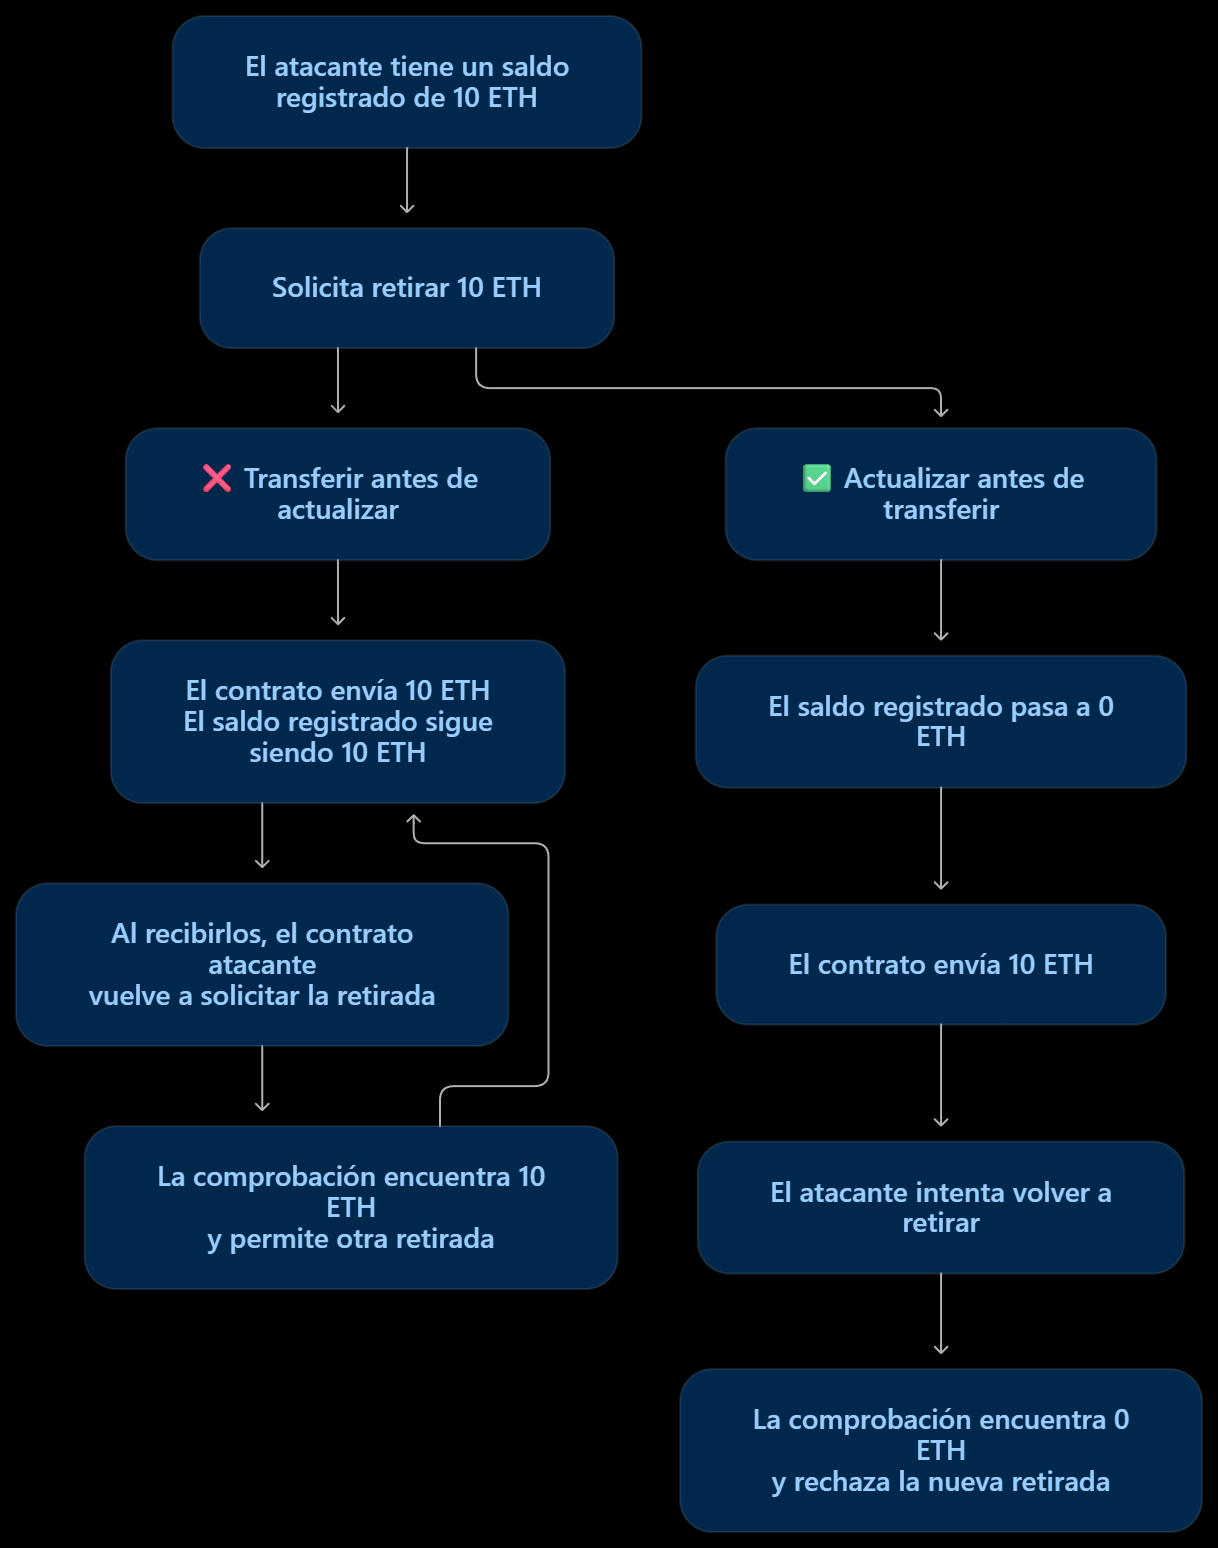
\includegraphics[width=\textwidth]{figures/ataqueReentrada-diagram.png}
    \label{fig:ataque-reentrada}
\end{figure}



\section{Validación de resultados}
\subsection{Validación a través del uso de la aplicación del sistema}
Tras el desarrollo del sistema de préstamos descentralizado, es necesario 
comprobar si cumple con los objetivos planteados y cubre los casos de uso 
definidos. 
Para ello, se ha realizado manualmente un flujo de uso de la interfaz de usuario y
se presentan pruebas mediante capturas de pantalla de la interfaz 
y registros en la herramienta \textit{Etherscan} para validar la ejecución de 
las transacciones y el correcto funcionamiento de los \glspl{smartcontract}
en la \gls{blockchain} de \gls{ethereum}.
Para comprender las siguientes imágenes es importante conocer 
los siguientes conceptos:

\begin{enumerate}
    \item \textbf{Wei:} En la red \gls{ethereum} es la unidad más pequeña de valor 
    para su criptomoneda \gls{eth}. Un \gls{eth} está compuesto por un total de 
    $10^{18}$ wei.
    \item Las cadenas de caracteres que comienzan por \texttt{'0x'} en la red 
    \gls{ethereum} están reservadas como direcciones que pueden apuntar a 
    usuarios, entidades o \glspl{smartcontract}.
    
\end{enumerate}


El \gls{op}~\ref{op:2} consiste en la unificación de las distintas funcionalidades 
del proyecto en una interfaz accesible a cualquier sujeto independientemente de su formación.
Los resultados se podrán ver a lo largo de la sección y se podrá apreciar que, aunque la 
interfaz sí reúne todas las funcionalidades del sistema, no se ha hecho hincapié en la
accesibilidad e intuitividad. 
Durante el desarrollo del proyecto se ha decidido aportar más esfuerzo en la funcionalidad 
dejando la evolución de la interfaz de usuario a un estado más \textit{amigable} para
trabajo futuro.

Para la validación de resultados del \gls{op}~\ref{op:1} se pueden evaluar los distintos objetivos secundarios:
\begin{enumerate}
    \item \textbf{\gls{os}~\ref{os:1}:} La aplicación solicita a \gls{metamask} la
    conexión de una cuenta y la autorización de las operaciones. La dirección
    permite asociar los préstamos a una cuenta. La figura~\ref{fig:metamask} muestra
    este acceso a la aplicación.

    \begin{figure}[H]
    \centering
    \caption{Ejemplo de inicio de sesión con MetaMask}
    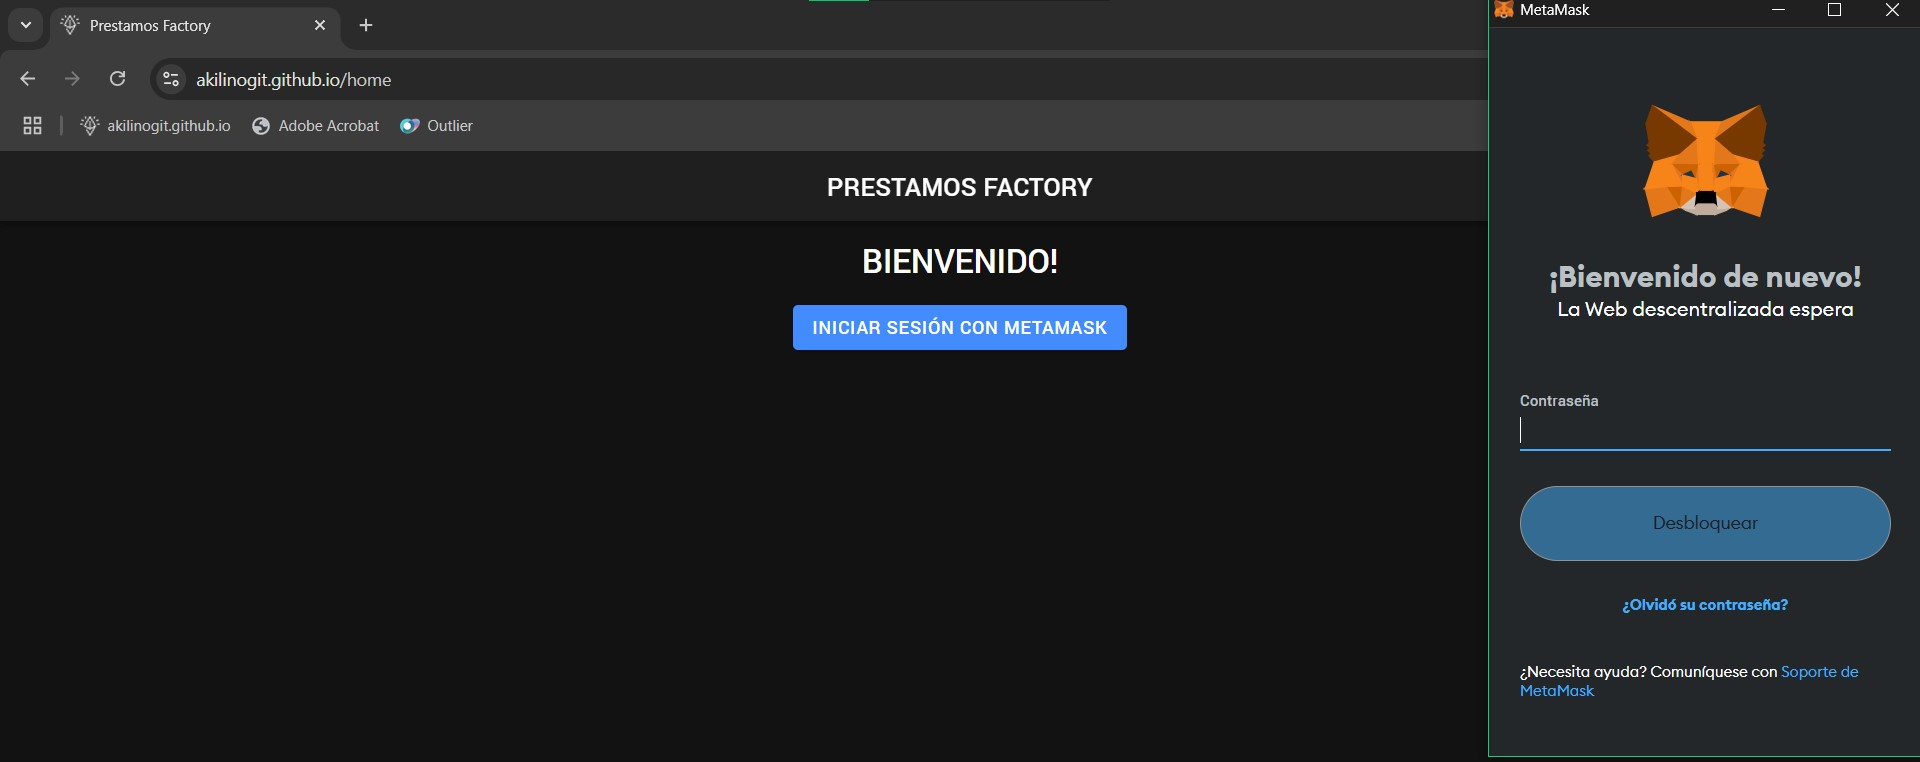
\includegraphics[width=\textwidth]{figures/resultados/metamask.jpg}
    \label{fig:metamask}
\end{figure}

    \item La utilización de \gls{metamask} no solo nos sirve para delegar 
    la identificación 
    sino también para delegar en una empresa externa la información que 
    identifica a 
    nuestros clientes, de forma que  no hace falta grabarla en la red.
    Esto nos ayuda con el \gls{os}~\ref{os:6} el cual busca este punto
    de unión. 
    Gracias a \gls{metamask} aunque existan cientos de operaciones económicas 
    reflejadas 
    en la red, sólo es posible comprobar la identidad de los participantes 
    de estas operaciones 
    a través de \gls{metamask} y las claves privadas de cada usuario.

    \item En el \gls{os}~\ref{os:2} se busca la eficiencia en la información y 
    las funciones del sistema para evitar el alto consumo de energía y \gls{gas} 
    a la hora 
    de ejecutar las transacciones en la red:

    Todas las funciones que tienen relación con la red son funciones muy atómicas 
    y sencillas evitando los grandes procesamientos de datos en la red aunque es 
    posible que la función que se encarga de comprobar los pagos de los contratos 
    de forma mensual pueda suponer una alta inversión por parte de la entidad
    financiera en caso de que tenga un volumen alto de préstamos, lo cual nos
    lleva a una posible actuación futura para limitar la cantidad de procesamiento 
    en esta acción.

    \item Haciendo referencia al \gls{os}~\ref{os:4} se adjuntan las siguientes
    imágenes del panel de control de la entidad prestamista en el que se muestran
    3 contratos de un usuario en curso antes y después de  la comprobación 
    mensual de los pagos de las cuotas.
    En ellas se pueden observar los distintos detalles:
    
    \begin{enumerate}
        \item El balance de la entidad después del pago de cuota del usuario
        aumenta correctamente
        \item Uno de los contratos no ha pagado correctamente la cuota 
        y se le ha aplicado automáticamente la penalización por impago.
        \item Uno de los contratos correctamente pagado ha reducido su deuda 
        restante y el número de cuotas restantes.
        \item En el caso del contrato que solo tenía una cuota restante, 
    ya no se muestra en la \gls{dapp} ya que no es necesario 
        replicar más esta información.
    \end{enumerate}
    Estas comprobaciones se pueden ver reflejadas con el cambio de información 
    correspondiente en la figura que muestra la información previa a la 
    comprobación mensual~\ref{fig:prechequeo} y tras la comprobación mensual 
    en la figura~\ref{fig:postchequeo}


\begin{figure}[H]
    \centering
    \caption{Información de contratos previa a la comprobación mensual en el recuadro amarillo y balance de la entidad prestamista en el recuadro blanco.}
    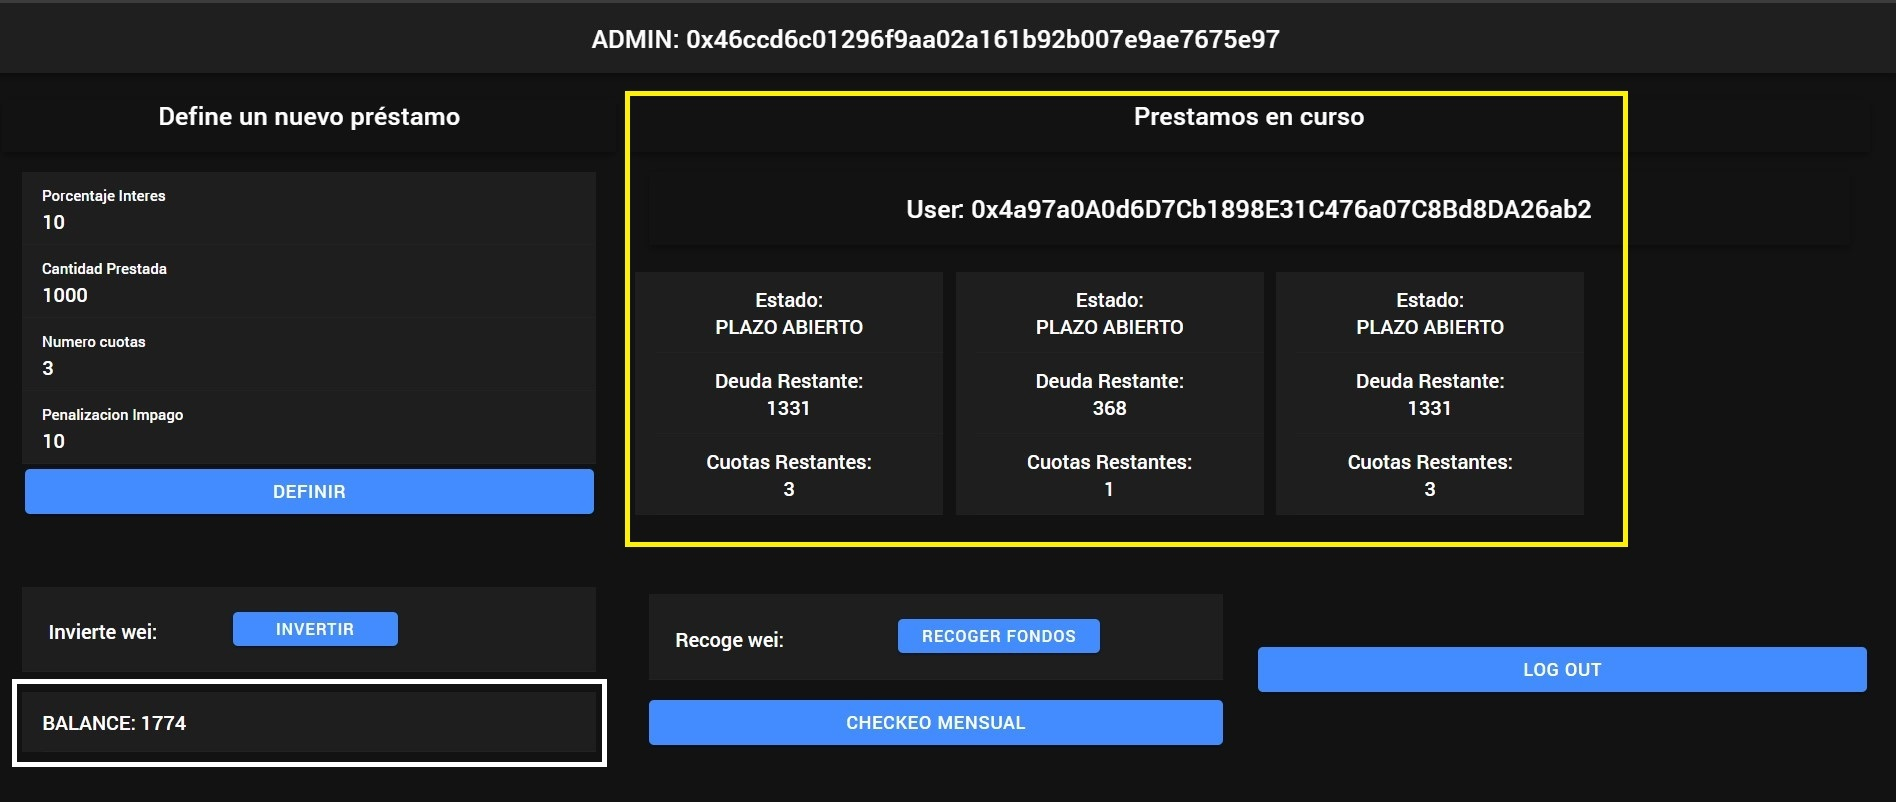
\includegraphics[width=\textwidth]{figures/resultados/prechequeo.jpg}
    \label{fig:prechequeo}
\end{figure}

\begin{figure}[H]
    \centering
    \caption{Información de contratos posterior a la comprobación mensual en el recuadro amarillo y balance de la entidad prestamista en el recuadro blanco.}
    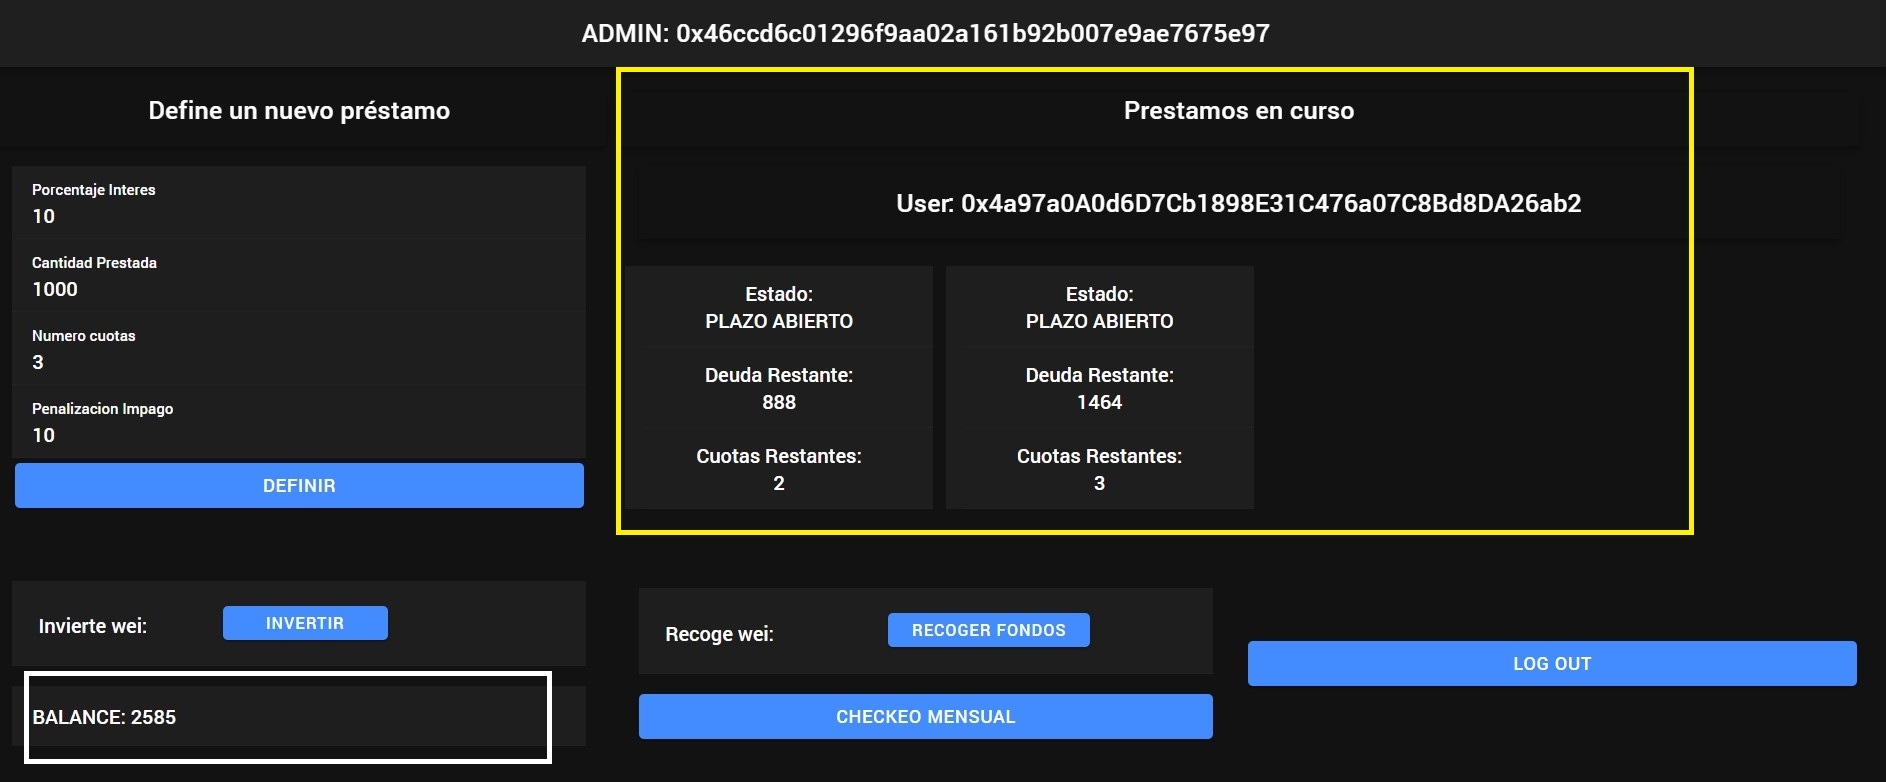
\includegraphics[width=\textwidth]{figures/resultados/postchequeo.jpg}
    \label{fig:postchequeo}
\end{figure}



Las últimas características declaradas junto con la posibilidad de que la 
organización del sistema pueda recibir los \gls{wei} del balance del sistema 
a través de la función \textit{Recoger Fondos} nos llevan al alcance del 
\gls{os}~\ref{os:7}, el cual busca encontrar la liquidez en este sistema.


\item En el \gls{os}~\ref{os:5} se contempla la posibilidad de personalizar 
los contratos accesibles para los distintos usuarios, esto se puede clasificar 
como inalcanzable para este proyecto debido a la necesidad de procesar
grandes cantidades de datos de clientes para poder crear un algoritmo y un 
sistema que cubra esta necesidad.

De momento existe la posibilidad de definir nuevos préstamos contratables en
el panel de control de la entidad prestamista.


\end{enumerate}

Para terminar de validar el \gls{op}~\ref{op:2} se adjunta captura de pantalla 
del panel de control del usuario en la figura~\ref{fig:paneluser} demostrando 
una interfaz unificada para el usuario.
        \begin{figure}[H]
    \centering
    \caption{Panel de control del usuario.}
    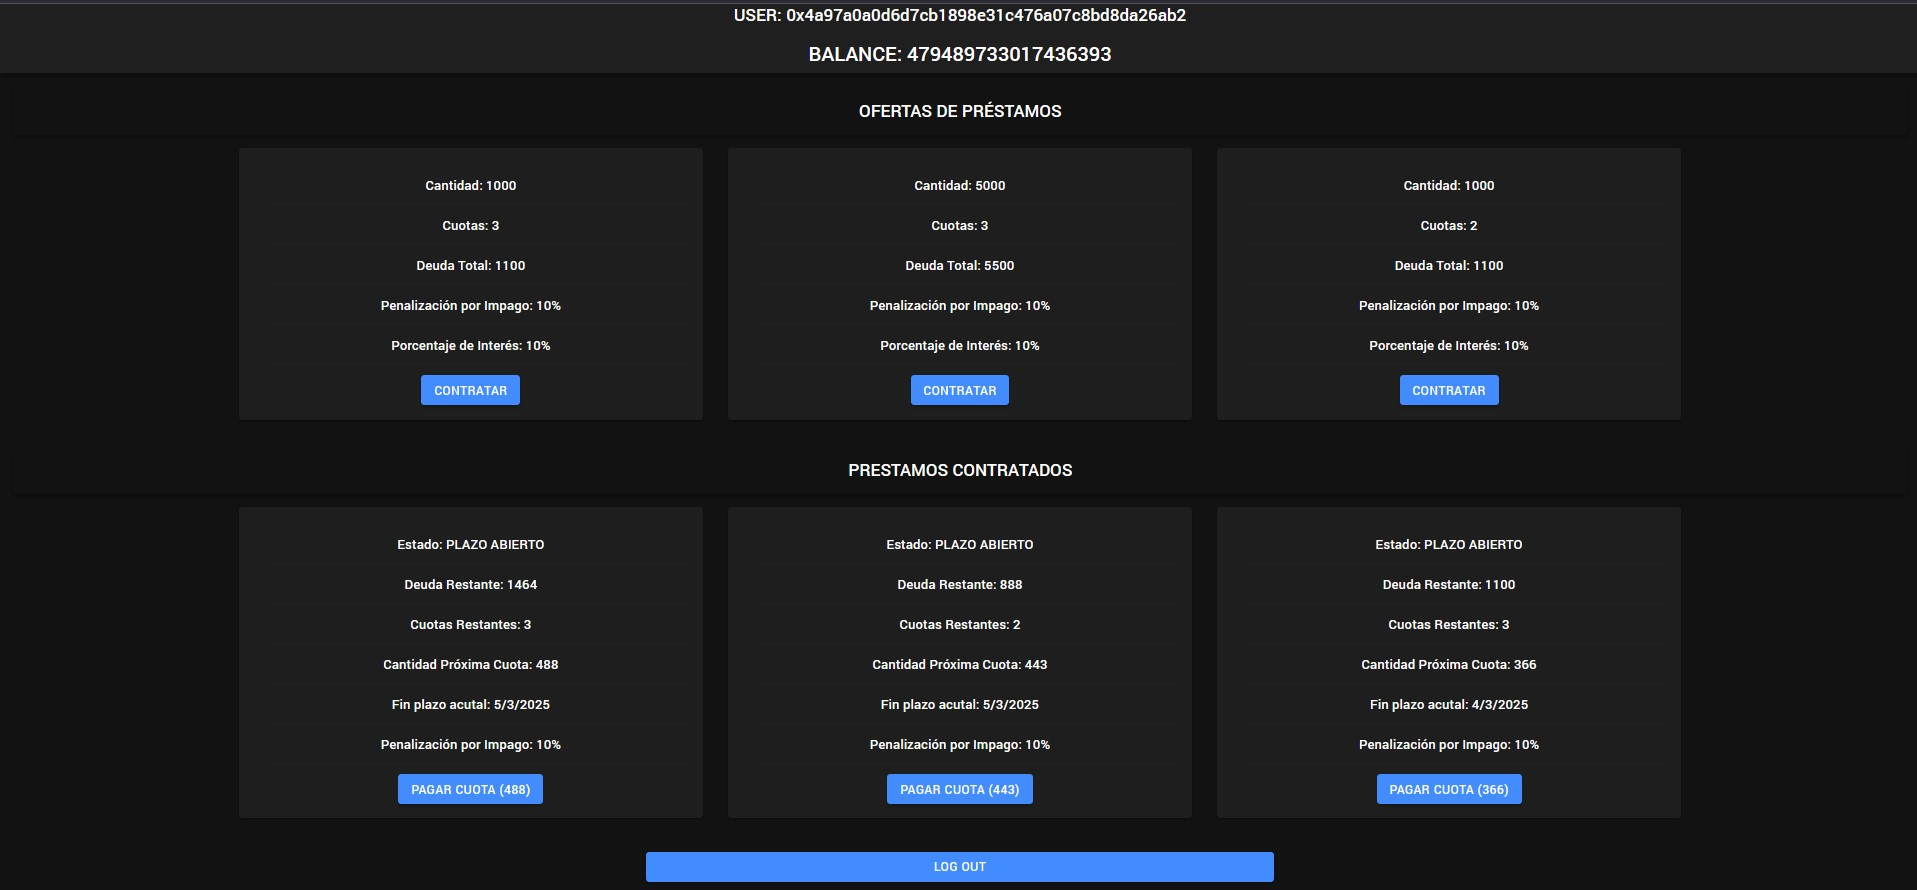
\includegraphics[width=\textwidth]{figures/resultados/paneluser.jpg}
    \label{fig:paneluser}
\end{figure}


Como última prueba de validación manual de este proyecto se realiza un ejemplo de 
contratación de préstamo adjuntando distintas capturas de la web
\href{https://sepolia.etherscan.io/}{Etherscan Sepolia} 
con las que se pueden comprobar distintos elementos relacionados con el proceso
que corroboran la veracidad del préstamo a través de la red 
\href{https://sepolia.dev/}{ Sepolia}.

\paragraph{Ejecución de préstamo de 1000~\gls{wei}}
\textbf{Contrato principal:} En la anterior figura~\ref{fig:postchequeo}
se puede comprobar que el balance del contrato principal es de 2585~\gls{wei}.

\textbf{Balance del usuario}: Después de la contratación del usuario,  
se puede ver a través de \href{https://sepolia.etherscan.io/}{Etherscan Sepolia}, 
tal y como se muestra en la figura~\ref{fig:Etherscan smart contract principal}, 
que:

    \begin{itemize}
        \item El balance del contrato ha disminuido 1000~\gls{wei}
        \item Se ha registrado una transacción de creación de contrato 
        (\textit{Contract Creation}), correspondiente al nuevo préstamo.
        \item Aunque debido al redondeo de la página aparezca otra transacción 
        de 0 \gls{eth}, viendo el balance se puede comprobar que es de 
        1000~\gls{wei} y han sido transferidos a la dirección del usuario.
    \end{itemize}

\begin{figure}[H]
    \centering
    \caption{Información de Etherscan del registro en la red SepoliaETH del 
    contrato inteligente principal}
    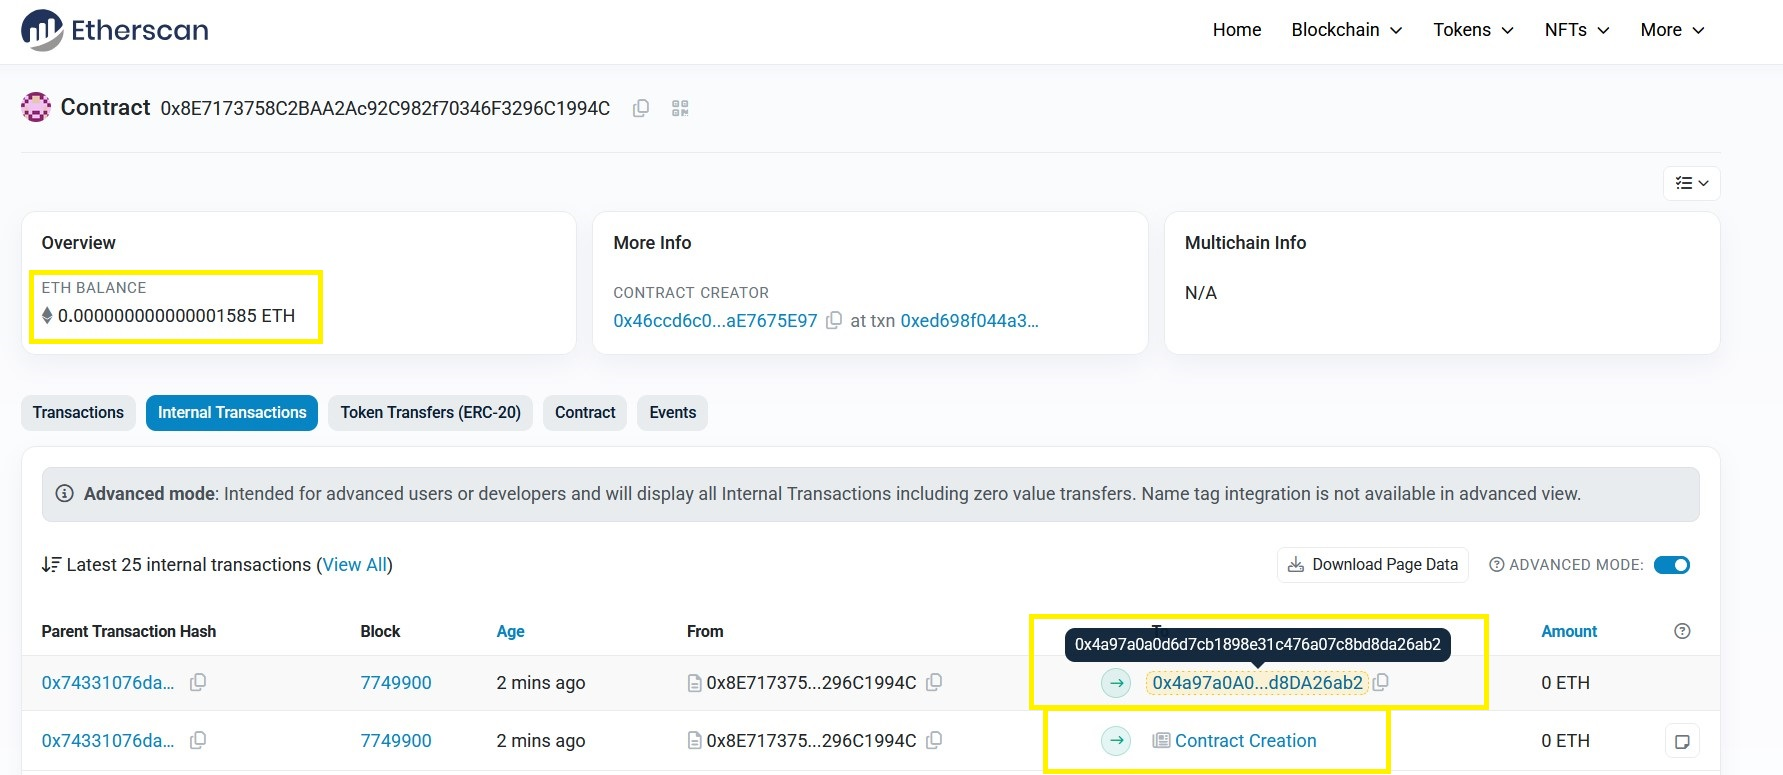
\includegraphics[width=\textwidth]{figures/resultados/createcontract.jpg}
    \label{fig:Etherscan smart contract principal}
\end{figure}

Se adjunta también otra captura de pantalla en la 
figura~\ref{fig:Etherscan comprobante de pago} de la información 
de la instancia generada del \gls{smartcontract} \textit{PrestamoCursando}

En la figura~\ref{fig:Etherscan comprobante de pago} también se puede observar
dentro del recuadro amarillo la primera transferencia recibida por parte del 
usuario con la cuota mensual. Esta cantidad de 366~\gls{wei} coincide correctamente
con el atributo \textit{Cantidad próxima cuota} del tercer préstamo contratado 
en el panel de usuario de la figura~\ref{fig:paneluser}.

Con esta comprobación de función de pago en 
\href{https://sepolia.etherscan.io/}{Etherscan Sepolia} 
se da por validado que todas las funciones del proyecto se reflejan en la red 
otorgando veracidad e inmutabilidad al proyecto.
\begin{figure}[H]
    \centering
    \caption{Registro en Sepolia en el que se puede ver una transacción o comprobante de pago Etherscan}
    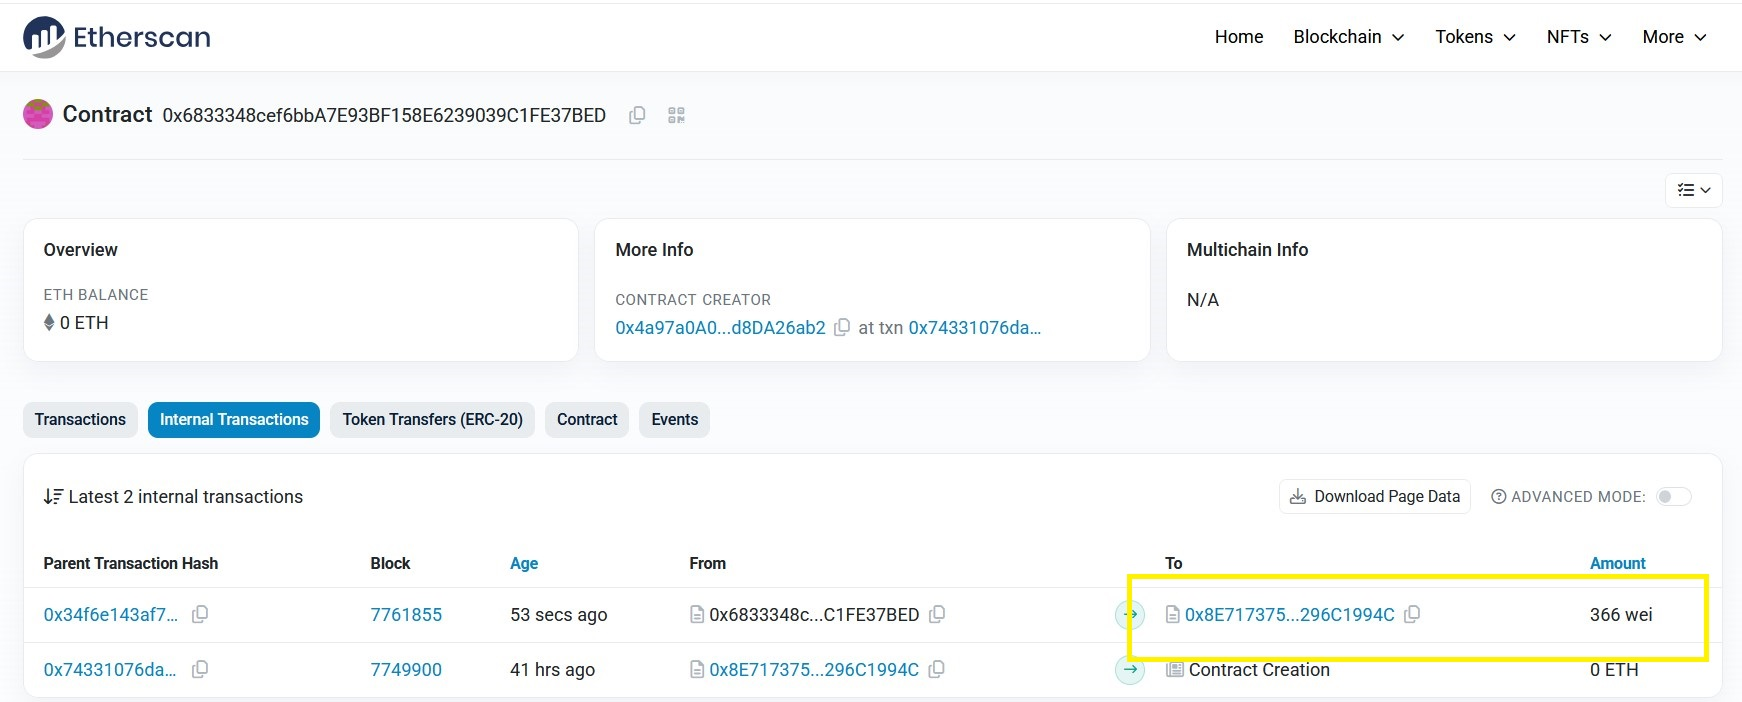
\includegraphics[width=\textwidth]{figures/resultados/pagoprestamo.jpg}
    \label{fig:Etherscan comprobante de pago}
\end{figure}


\subsection{Pruebas con Mocha}
Ya se ha visto el correcto funcionamiento de la aplicación a través de la
interfaz de usuario y la verificación de las transacciones en la red.
Pero para garantizar el correcto funcionamiento de los \glspl{smartcontract} en
situaciones distintas al correcto uso de la aplicación, 
se han desarrollado distintas pruebas unitarias utilizando la herramienta
\hyperref[sec:mochasection]{entorno de pruebas Mocha}.

Estas pruebas tienen como objetivo:
\begin{enumerate}
    \item Comprobar el funcionamiento de los contratos inteligentes.
    \item Verificar que las operaciones de préstamos funcionan correctamente.
    \item Detectar errores en condiciones normales y situaciones no permitidas.
    \item Comprobar las restricciones de acceso y los cambios de estado.
\end{enumerate}

\paragraph{Red de pruebas local:}
Para evitar utilizar una red pública se han desplegado los contratos sobre una red local utilizando la herramienta Ganache~\cite{[19]}.
Esto evita que aparezcan transacciones de prueba exponiendo información sensible del funcionamiento del  sistema en la red pública y 
permite la repetición de escenarios que son difíciles de reproducir en un entorno real, como que un usuario no pague su cuota mensual y se le aplique la penalización correspondiente.
\paragraph{Cuentas utilizadas para las pruebas:}
La herramienta de creación de red local virtual es la encargada de generar distintas cuentas con las que interactuar en la red.
Se han utilizado 3 cuentas para realizar las pruebas unitarias:
\begin{enumerate}
    \item Una cuenta propietaria del sistema
    \item Dos cuentas de usuario que solicitan el préstamo
\end{enumerate}
\paragraph{Contratos inteligentes puestos a prueba:}
Las pruebas se han hecho sobre el motor de este sistema, es decir, sobre los
\glspl{smartcontract} que definen el funcionamiento del sistema de préstamos.
Estos contratos se pueden ver en el anexo ~\ref{anexo:smartcontracts} y son los 
ya comentados \textit{PrestamosFactory} y \textit{PrestamoCursando}.

\paragraph{Tecnología de las pruebas:}
Las pruebas se han desarrollado utilizando JavaScript, el entorno de pruebas Mocha y
el módulo \texttt{assert} de Node.js para las aserciones.
Estas pruebas se pueden encontrar en el anexo~\ref{anexo:mochatest}.

\paragraph{Desarrollo de las pruebas: Variables previas y condiciones iniciales:}
Previo al desarrollo puro de las pruebas, antes de cada ejecución se deben dar las condiciones iniciales para que las pruebas puedan ejecutarse correctamente.
El proceso de preparación de las pruebas consiste en desplegar los contratos en la red local y establecer las condiciones iniciales para cada prueba.
Para ello se han realizado los siguientes pasos:
\begin{enumerate}
    \item \textbf{Compilación en local de los contratos inteligentes:} A través de la
    herramienta \textit{Truffle} se compilan los \glspl{smartcontract} 
    previamente para que la red sea capaz de entender sus funciones.
    Esta compilación genera un archivo .json con las funciones del \gls{smartcontract} 
    parametrizadas para que la red sea capaz de interactuar con él.
    \item \textbf{Obtención de cuentas:} Se obtienen las cuentas necesarias para realizar las pruebas.
    \item \textbf{Despliegue del contrato en la red:} En el desarrollo de las pruebas se hace uso del archivo .json de la compilación y se despliega el contrato a testear en la red local de pruebas.
            \begin{lstlisting}[language=Solidity, caption={Despliegue de contrato en la red local}]
                    describe('Prestamos factory test', () => {

                    before( async() => {  
                        accounts = await web3.eth.getAccounts();
                        factory = await new web3.eth.Contract(prestamosFactoryBuild.abi)
                            .deploy({data: prestamosFactoryBuild.evm.bytecode.object})
                            .send({ from: accounts[0], gas: 6721975});
                        
                        console.log('contract address:'+ factory.options.address);
                        console.log('Owner: ' + accounts[0]);
                        
                        
                    } );

                \end{lstlisting}

    \item \textbf{Establecimiento del estado inicial:} En el caso de las pruebas para
    los \textit{PrestamoCursando}, se establecen primero las variables previas
    necesarias para la contratación de un préstamo.
    Estas son:
    \begin{enumerate}
        \item \textbf{Introducción de fondos:} El sistema de préstamos necesita
        fondos previos para que se le puedan solicitar préstamos.
        \item \textbf{Creación de un tipo de préstamo:} Se crea un tipo de
        préstamo con las características necesarias para la prueba.
        \item \textbf{Creación de contratos de préstamo y obtención de sus
        direcciones:} De esta manera se obtiene la forma de acceder a los
        contratos sobre los que se ejecutarán las pruebas.
    \end{enumerate}
    
\begin{lstlisting}[language=Solidity, caption={Parametrización de préstamos en curso}]
    describe('Prestamos Cursando test', async () => {
    //INICIALIZAR PRESTAMOS EN CURSO
    before(async() => {  
        //Inicializar cuentas
        accounts = await web3.eth.getAccounts();
        
        
        //Inicializar contract factory
        factory = await new web3.eth.Contract(prestamosFactoryBuild.abi)
            .deploy({data: prestamosFactoryBuild.evm.bytecode.object})
            .send({ from: accounts[0], gas: 6721975});
            

        //Invertir para poder crear nuevos contratos
        await factory.methods.invertir().send({
                from: accounts[0],
                value: web3.utils.toHex(10000)
            });
        //Definir préstamo
        await factory.methods.definirPrestamo(10,1000,2,10).send({from: accounts[0],
            gas: web3.utils.toHex(2000000)});
        //Contratar préstamos
        await factory.methods.contratarPrestamo(accounts[1],0).send({from: accounts[1],
            gas: web3.utils.toHex(2000000)});
        await factory.methods.contratarPrestamo(accounts[2],0).send({from: accounts[2],
            gas: web3.utils.toHex(2000000)});

        [prestamo1address]=await factory.methods.verContratos(accounts[1]).call({from: accounts[1]});
        [prestamo2address]=await factory.methods.verContratos(accounts[2]).call({from: accounts[2]});
        
        prestamo1 = await new web3.eth.Contract(prestamoCursandoBuild.abi,prestamo1address);
        prestamo2 = await new web3.eth.Contract(prestamoCursandoBuild.abi,prestamo2address);
        
    });
    \end{lstlisting}

    \item \textbf{Descripción de las pruebas:} El contenido de las pruebas se puede ver en
    los dos ficheros del anexo ~\ref{anexo:mochatest} y se describen a 
    continuación:
            \begin{enumerate}
                \item \textbf{Pruebas del \texttt{PrestamosFactory}}

                En \path{test_prestamos_factory.js} se comprueba principalmente el \textbf{funcionamiento de PrestamosFactory y sus restricciones}:

                \begin{enumerate}
                    \item \textbf{Despliegue del contrato}: se verifica que el \texttt{PrestamosFactory} se despliega correctamente y obtiene una dirección.
                    \item \textbf{Control de acceso}: se comprueba que determinadas funciones únicamente pueden ser ejecutadas por el \texttt{owner}.
                    \item \textbf{Ingreso de fondos}: se comprueba que \texttt{invertir()} incrementa correctamente el saldo del Factory.
                    \item \textbf{Consulta de saldo}: se verifica que \texttt{getBalance()} devuelve el saldo real del contrato.
                    \item \textbf{Estado inicial}: se comprueba que inicialmente no existen clientes, tipos de préstamo ni préstamos en curso.
                    \item \textbf{Retirada de fondos}: se verifica que \texttt{recolectarFondos()} reduce correctamente el saldo del Factory.
                    \item \textbf{Validación de parámetros}: se prueban valores incorrectos para los porcentajes de intereses y penalizaciones, comprobando que las operaciones son rechazadas.
                    \item \textbf{Creación de tipos de préstamo}: se comprueba que \texttt{definir\allowbreak{}Prestamo()} crea correctamente un nuevo producto y genera el evento correspondiente.
                    \item \textbf{Consulta de tipos de préstamo}: se verifica que los datos almacenados coinciden con los valores introducidos.
                    \item \textbf{Contratación de préstamos}: se comprueba tanto la contratación correcta como situaciones en las que la operación debe fallar.
                    \item \textbf{Consulta de préstamos de un usuario}: se verifica que \texttt{ver\allowbreak{}Contratos()} devuelve los contratos correspondientes.
                    \item \textbf{Intento de eliminar un préstamo no finalizado}: se comprueba que esta operación no está permitida.
                \end{enumerate}

                \item \textbf{Pruebas del \texttt{PrestamoCursando}}

                El segundo archivo prueba el \textbf{ciclo de vida de un préstamo individual}.

                Se parte de una situación preparada con:

                \begin{enumerate}
                    \item Factory desplegado.
                    \item Fondos introducidos.
                    \item Tipo de préstamo creado.
                    \item Dos préstamos contratados por usuarios diferentes.
                \end{enumerate}

                A partir de ahí se prueban:

                \begin{enumerate}
                    \item \textbf{Control de acceso a la información}: un usuario diferente al prestatario no puede consultar la información privada del préstamo.
                    \item \textbf{Consulta de información del préstamo}: se comprueban importe prestado, deuda, cuota mensual, número de cuotas, estado, prestatario, etc.
                    \item \textbf{Restricción temporal}: se comprueba que no se puede realizar el chequeo mensual antes de que haya transcurrido el tiempo establecido.
                    \item \textbf{Pago de una cuota}: se realiza un pago y se comprueba que:
                    \begin{enumerate}
                        \item[a)] disminuye el número de cuotas restantes;
                        \item[b)] disminuye la deuda;
                        \item[c)] cambia el estado del préstamo.
                    \end{enumerate}
                    \item \textbf{Transferencia de fondos}: se verifica que el dinero pagado vuelve correctamente al \texttt{PrestamosFactory} y que su balance es el esperado.
                    \item \textbf{Chequeo mensual}: se simula el paso del tiempo y se comprueba que el chequeo:
                    \begin{enumerate}
                        \item[a)] actualiza el estado del préstamo;
                        \item[b)] aplica una penalización al préstamo que no ha sido pagado.
                    \end{enumerate}
                    \item \textbf{Finalización del préstamo}: se paga la última cuota y se comprueba que el préstamo pasa al estado de finalizado.
                    \item \textbf{Eliminación de préstamos finalizados}: después del chequeo mensual se comprueba que el contrato finalizado deja de aparecer entre los préstamos activos del usuario y que se actualiza la lista de clientes.
                \end{enumerate}
            \end{enumerate}

    \item \textbf{Comprobación de las pruebas} Tras la ejecución de las pruebas, se comprueba que los resultados obtenidos son los esperados y que el sistema funciona correctamente.
     Para ello se utilizan las funciones de aserción de Node.js, que permiten comparar los resultados obtenidos con los esperados y generar un informe de las pruebas realizadas.
       \end{enumerate}
    
\paragraph{Resultados} Tras el desarrollo y ejecución de las pruebas se puede comprobar que el sistema funciona correctamente y que se cumplen los objetivos planteados.
    A su vez se han encontrado 2 situaciones que no se contemplaban en el diseño inicial.
\begin{enumerate}
    \item La función \texttt{setIndex} actualiza el índice de un préstamo.
    En el código del anexo está restringida mediante \texttt{onlyContractFactory},
    que comprueba que el emisor sea el contrato principal y tuviese
        el archivo compilado del contrato podría acceder directamente a esta 
        función y simular que es uno de los contratos en curso 
        y modificar el índice de los contratos de un usuario pudiendo quedar 
        invisibles.
        \item La función que comprueba mensualmente el estado de todos los 
        contratos del sistema se demora más segundos de los que el tiempo de espera de Mocha tiene por defecto por lo que se ha tenido que aumentar.
\end{enumerate}

\subsection{Validación del proyecto después de pruebas}
Durante la ejecución de las pruebas de este proyecto y la simulación de un entorno real se ha visto que un sistema como este puede llegar a niveles de producción
en un entorno real. Dejando aparte la necesidad de un desarrollo futuro para
añadir actores y elementos necesarios para un sistema de préstamos real
a nivel técnico se afirma que la tecnología es viable.

\subsection{Viabilidad económica}
Tras estudiar los gastos de \gls{gas} en los registros de 
\href{https://sepolia.etherscan.io/}{Etherscan Sepolia} se puede comprobar 
que los gastos de contratar un préstamo
dependen mucho del precio del \gls{gas} en el momento de contratación, 
el cual varía de forma muy dinámica dependiendo de la congestión de la red.
En el proceso de validación se han ejecutado
 transferencias de préstamo con costes desde 0,46 dólares hasta 30,49 dólares.
 Esto puede crear un cuello de botella de entrada de préstamos en caso de que 
 se dependa en exceso de esta variable obligando 
a la gestión del sistema a retrasar contratos y operaciones cuando el coste 
sea muy alto o directamente pasar los costes a los clientes.
Por otro lado, independientemente de esta variable, a nivel técnico se ha 
comprobado que en el momento en el que se comprueba si todos los préstamos
 han sido pagados o no
la cantidad de procesamiento aumenta linealmente por el número de contratos 
en el sistema, sumando esto a un alto coste del gas se podría crear un bloqueo
total del sistema,
por lo que sería obligatorio optimizar la forma en la que se realiza este 
chequeo.



\include{secciones/resultadosdeldesarrollo}
\chapter{Conclusiones}

%%RESUMEN E INTRODUCCIÓN

En este Proyecto Fin de Grado se ha desarrollado un sistema de préstamos 
descentralizado basado en la red \gls{ethereum}. 
Tras el desarrollo se pueden llegar a las siguientes conclusiones:
\begin{itemize}
     \item Se puede afirmar que se ha obtenido 
una aplicación capaz de conectarse con una red \gls{blockchain} y de realizar 
transacciones en ella.

Gracias al registro de estas transacciones y cierta lógica aplicada 
a esta información, se puede componer un sistema de creación y control de préstamos 
digitales en el que el contrato de nuevos préstamos queda totalmente automatizado.

     \item Es posible unificar todas las herramientas de gestión dentro de la una interfaz de 
usuario cubriendo todas las conexiones necesarias con la red de \gls{ethereum} 
y capaz de ordenar la ejecución en la red las operaciones necesarias para la 
gestión de un sistema de préstamos digitales.

     \item Aunque para un sistema aplicado en la vida real hiciera falta 
     la implementación de distintos desarrollos, los \glspl{smartcontract} 
     desplegados en la red definen correctamente la lógica 
     aplicada a la información necesaria para la realización de préstamo.

     \item El correcto registro de esta información en la red \gls{blockchain} 
     proporciona al sistema las características de seguridad, inmutabilidad y 
     veracidad necesarias para un sistema de esta índole.

     \item Exite un plan de validación que verifica las capacidades descritas 
     para este sistema.

     \item Tras un estudio del impacto social se puede concluir que la adopción 
     de tecnologías \gls{defi} y \gls{smartcontract} tiene el potencial de transformar
     el acceso a servicios financieros y dependiendo del uso que se de a esta 
     tecnología se puede aumentar o disminuir la inclusión financiera.
\end{itemize}




\section{Trabajo futuro}

En el desarrollo de este proyecto se ha podido comprobar que un sistema de prestamos
descentralizado es posible, pero, para que un proyecto como este llegue a una situación
de producción real es necesario realizar una serie de desarrollos para cumplir con 
necesidades básicas en un sistema de préstamo real.

Se considera la más importante la adopción de garantías de impago, esta carencia del 
proyecto se tiene en cuenta en el Caso de uso futuro \hyperlink{cu:garantia}{CU12} :  Garantía de devolución en 
caso de impago,
aunque actualmente el sistema sea capaz de penalizar los impagos, no se garantiza recuperar
el capital prestado, para ello se pueden desarrollar dos casos de uso:
\begin{itemize}
     \item Creación de sistema de colaterales: en un futuro será de obligado 
     cumplimiento que el usuario que solicite un prestamo añada al sistema 
     alguna garantía, la cual puede estar en forma de \gls{nft}, y en caso 
     de que el usuario se declare en situación de impago, este \gls{nft} pasaría 
     automaticamente a ser propiedad del sistema
     \item Creación de sistema de avales: En situaciones en los que el usuario 
     no pueda añadir esa garantía o colateral se podrá añadir al contrato un tercero 
     capaz de añadir un colateral al contrato e incluso encargarse de las cuotas en 
     caso de que el usuario principal no lo haga
\end{itemize}

El nuevo sistema de garantías también debera incluir un sistema de validación de 
solvencia, tal y como se habla en el Caso de uso futuro \hyperlink{cu:garantia}{CU14}, lo que aportará 
mayor solided a la garantía de devolución.

Durante los tests de funcionamiento del sistema se pudo comprobar las ineficencias 
de código en la red. Sobretodo evitar recorrer todos los contratos existentes 
una vez al mes para comprobar si han sido pagados o no. 

Para ello el sistema se puede 
apoyar en elementos externos a la red, como una base de datos temporal en la que 
puede 
quedar reflejado cada pago de la mensualidad y mensualmente ejecutar las 
penalizaciones en la red con los contratos que no aparecen en esta base de datos,
aunque sea una base de datos externa, su uso no rompe con ninguna característica 
en las que se apoya el sistema ya que solo sería un apoyo técnico, 
manteniendo siempre 
reflejado en la red la situación financiera del sistema.

Como se pudo ver en la sección de~\ref{subsec:limitaciones-legales}, durante 
el desarrollo del proyecto, la Unión Europea abrueba un nuevo Reglamento Europeo de 
criptoactivos, por lo que para una producción real es de obligado cumplimiento 
cubrir esta normativa.

En el~\ref{op:2} se habla de que este proyecto debe contener una interfaz de usuario 
unificada, facil e intuitiva. Aunque si se ha desarrollado una interfaz unificada 
sería necesario crar una intefaz más intuitiva al usuario.

Con menos prioridad se deberán desarrollar sistemas que utilicen \gls{oraculo} 
tal y como se habla en el Caso de uso Futuro \hyperlink{cu:garantia}{CU13}, este sistema junto a la comprobación 
de solvencia económica pueden servir para una correcta definición de  los tipos de 
prestamo y condiciones disponibles en el sistema.





\section{Impactos sociales y ambientales del desarrollo de este sistema a gran escala}

La adopción masiva de un sistema de préstamos descentralizado basado en blockchain y 
contratos inteligentes podría generar importantes transformaciones en el ámbito financiero y social.
La eliminación de intermediarios permitiría un acceso más democrático a los servicios financieros,
especialmente en regiones con sistemas bancarios limitados o restrictivos.

Sin embargo, este modelo también presenta retos significativos en términos de inclusión digital,
     regulación y sostenibilidad ambiental.

\subsection{Impactos sociales}
Sin embargo,
la reducción de intermediarios no garantiza por sí sola una mayor
inclusión financiera. Su impacto social dependería de las condiciones
de acceso al crédito, de las competencias digitales de los usuarios
y de los mecanismos de protección disponibles~\cite{oecd2024defi}.

\begin{enumerate}
     \item La posibilidad de otorgar préstamos sin la necesidad de bancos tradicionales
      podría beneficiar a millones de personas no bancarizadas en economías emergentes.
       Sin embargo, la \acrfull{ocde} señala que el acceso a estos servicios dependería del
        conocimiento en el uso de criptomonedas, \gls{wallet} digitales y plataformas \gls{defi}
         y  lo que podría aumenter la brecha digital entre quienes dominan estas herramientas
          y quienes no. A demás, la \acrfull{ocde} también señala que la responsabilidad del usuario
          sobre sus propios activos dificultan la utilización de estos.
          Por tanto,
    el acceso técnico a una plataforma no equivale a una inclusión
    financiera efectiva. En el sistema desarrollado, sería necesario
    facilitar la comprensión de su funcionamiento y del uso de
    una \gls{wallet} para reducir estas barreras~\cite{oecd2024defi}.

     \item La descentralización del sistema podría entrar en conflicto con regulaciones financieras
      existentes. Gobiernos y bancos centrales podrían imponer restricciones al uso de plataformas DeFi,
       especialmente en países donde el control financiero es una herramienta de política económica.
        Además, la anonimidad en las transacciones podría plantear problemas relacionados con el
         financiamiento ilícito si no se establecen mecanismos de verificación de identidad adecuados.

     \item La automatización de los préstamos a través de contratos inteligentes podría reducir la
      demanda de intermediarios financieros, afectando a trabajadores del sector bancario y generando
       resistencia por parte de instituciones tradicionales. Sin embargo, también abriría oportunidades
        en nuevas áreas tecnológicas, creando demanda de profesionales en blockchain, ciberseguridad y
         programación de contratos inteligentes.
     \item \textbf{Acceso efectivo al crédito.}
    El BIS advierte que muchos préstamos DeFi requieren aportar
    garantías cuyo valor supera el importe solicitado. Esta
    exigencia limita su utilidad para personas que carecen de
    patrimonio previo y necesitan financiación~\cite{aramonte2022defi}.

\end{enumerate}


\subsection{Impactos ambientales}
 
\begin{enumerate}
     \item Ethereum, aunque ha reducido su impacto ambiental tras su transición de Proof of Work (\gls{pow}) a Proof of Stake (\gls{pos}),
      sigue dependiendo de una infraestructura global de nodos y validadores que consumen energía.
       A gran escala, este sistema de préstamos podría contribuir al aumento de la demanda energética de los centros de datos y redes descentralizadas,
        lo que requeriría soluciones de eficiencia energética y compensación de emisiones.
 \end{enumerate}

 Si bien un sistema de préstamos descentralizado tiene el potencial de democratizar el acceso financiero y reducir costos,
  también presenta desafíos sociales y ambientales que deben abordarse antes de una implementación a gran escala.
   Para mitigar estos impactos, sería fundamental desarrollar estrategias de educación digital y
    establecer mecanismos de regulación equilibrados para  mejorar la eficiencia energética del sistema.

 Solo con un enfoque responsable y sostenible se podrá garantizar que este tipo de innovación beneficie a la sociedad sin comprometer
  el bienestar ambiental.

\subsection{Objetivos de desarrollo sostenible. Agenda 2030}
 La Agenda 2030 para el Desarrollo Sostenible es un plan global adoptado en 2015 por los Estados Miembros de la ONU con el objetivo de erradicar la pobreza, proteger el planeta y garantizar la prosperidad para todas las personas. Para lograrlo, se establecieron 17 \gls{ods}, que abarcan áreas clave como la educación, la igualdad de género, la acción climática, la innovación y el crecimiento económico, entre otras.

Estos objetivos buscan equilibrar el desarrollo social, económico y ambiental, promoviendo un modelo sostenible que asegure el bienestar de las generaciones actuales y futuras. Además, llaman a la colaboración entre gobiernos, empresas y la sociedad civil para alcanzar metas concretas antes del año 2030.

 En la figura 4.1 se pueden ver estos objetivos:

   \begin{figure}[H]
    \centering
    \caption{Objetivos de desarrollo sostenible de la agenda europea para 2030}
    
\includegraphics[width=\textwidth]{figures/2030.jpg}
    \label{fig:2030}
\end{figure}

Se puede concluir que este proyecto tiene un gran potential de influir 
positivamente en los objetivos relacionados en el ámbito financiero como los 
\gls{ods} 8 y 9 ya que supone la creación de una nueva infraestructura 
en el desarrollo de actividades económicas favoreciendo nuevas oportunidades de 
crecimiento económico.


El desarrollo de plataforma \gls{defi} tiene un gran potencial en la reducción de 
desigualdades y la aplicación de justicia social (\gls{ods} 10), la cuestión es
que el desarrollo de este potencial viene directamente correlacionado con el uso
que se le dé a esta tecnología pudiendo desarrollarse en una dirección opuesta a estos
\gls{ods}, si no se combate la brecha digital y se evita la creación de barreras articifiales pueden aumentar
por parte de los desarrolladores de esta tecnologías, 
las desigualdades y la injusticia social aumentarían todavía mas en vez de reducirse.

Algo parecido pasa con el \gls{ods} 16: la transparencia de las transacciones en un 
entorno descentralizado suponen una clara exposición de injusticias o malversaciones
realizadas en la red aunque esta característica pierde toda valided cuando se hace
un mal uso de la justicia y suceden eventos en los que se aprecia que 
\enquote{la justicia NO es igual para todos}

En el apartado ambiental (\gls{ods} 11, 12 y 13), aunque, es cierto, que tras el cambio de validación de 
bloques en la red a través de puro procesamiento y consumo eléctrico (\gls{pow})
por un sorteo en base a las aportaciones de capital en la red (\gls{pos}) se redujo
de manera drástica el consumo de electricidad, sigue habiendo otros problemas como 
la gestión de residuos de la infraestructura de la red.
Aunque volvemos a lo mismo que los apartados anteriores, siempre se puede utilizar
el aumento de productividad y capital en paliar los efectos adversos que este 
sistema incide en el ecosistema, todo depende del uso que se quiera dar a la 
tecnología.


\appendix
\chapter{Código fuente de los contratos inteligentes}
\label{anexo:smartcontracts}

En este anexo se presenta el código fuente de los contratos inteligentes desarrollados para el sistema de préstamos descentralizado basado en la red Ethereum.

\section{PRESTAMOS\_FACTORY.sol}

El archivo \path{PRESTAMOS_FACTORY.sol} incluye el contrato principal
\texttt{PrestamosFactory}, encargado de gestionar los tipos de préstamo y la
creación de nuevos contratos, y el contrato \texttt{PrestamoCursando}, que representa
un préstamo individual en curso.

\lstinputlisting[
    language=Solidity,
    caption={Código fuente de PRESTAMOS\_FACTORY.sol},
    label={lst:prestamos-factory}
]{smart contracts/PRESTAMOS_FACTORY.sol}

\chapter{Código fuente de las pruebas}
\label{anexo:mochatest}

En este anexo se incluye el código fuente de  las pruebas desarrolladas sobre los smart contract.



\section{test\_prestamos\_cursando.js}

Este archivo contiene las pruebas destinadas a verificar el comportamiento relacionado con los préstamos cursando.

\lstinputlisting[
    language=JavaScript,
    caption={Pruebas de prestamos cursando},
    label={lst:test-prestamos-cursando}
]{smart contracts/test_prestamos_cursando.js}


\section{test\_prestamos\_factory.js}

Este archivo contiene las pruebas destinadas a verificar el funcionamiento del Prestamos Factory.

\lstinputlisting[
    language=JavaScript,
    caption={Pruebas del contrato PRESTAMOS\_FACTORY},
    label={lst:test-prestamos-factory}
]{smart contracts/test_prestamos_factory.js}

\end{document}
